\documentclass[article]{jss}

\usepackage{amsmath,amssymb,amsfonts,amsthm}
\usepackage{bm}
\newtheorem{definition}{Definition}
\usepackage{booktabs}
\usepackage{graphicx}
\usepackage{tikz}
\usetikzlibrary{positioning,arrows.meta,fit,backgrounds,shapes.geometric}

%% -- pretty printing ------------------------------------------------
\newcommand{\pkgversion}{1.0.0.1.0}
\newcommand{\vcldversion}{1.0.0}

%% -- math shorthands ------------------------------------------------
\newcommand{\Reals}{\mathbb{R}}
\newcommand{\bX}{\bm{X}}
\newcommand{\bU}{\bm{U}}
\newcommand{\bu}{\bm{u}}
\newcommand{\cnd}{\,;\,}
\DeclareMathOperator{\diag}{diag}

%% -- declarations for jss.cls ---------------------------------------
\author{Thomas Nagler\\Ludwig-Maximilians-Universit\"at M\"unchen \And
        Thibault Vatter\\HES-SO Geneva}
\Plainauthor{Thomas Nagler, Thibault Vatter}

\title{\pkg{rvinecopulib}: A Fast and Comprehensive Implementation of Vine
       Copula Models in \proglang{C++} and \proglang{R}}
\Plaintitle{rvinecopulib: A Fast and Comprehensive Implementation of Vine
            Copula Models in C++ and R}
\Shorttitle{\pkg{rvinecopulib}: Vine Copula Models in \proglang{C++} and \proglang{R}}

\Abstract{
  Vine copulas decompose a multivariate distribution into a cascade of
  bivariate building blocks and have become a standard tool for flexible
  dependence modeling in moderate to high dimensions.  The \proglang{R}
  software that made them accessible has not kept pace with the methodology:
  the package documented in this journal a decade ago has been archived, its
  successor is in maintenance only, and both confine vine models to continuous
  data, user-supplied pseudo-observations, a fixed catalogue of parametric pair
  copulas, and a single structure-selection heuristic.  We present
  \pkg{rvinecopulib}, an \proglang{R} package built on \pkg{vinecopulib}, a
  header-only \proglang{C++17} library.  A vine structure is analysed once and
  the resulting index tells every subsequent algorithm --- fitting, density
  evaluation, simulation, the Rosenblatt transform, and the analytic derivative
  cascade --- exactly which conditional distribution functions it must compute
  and which it may skip.  The package is faster than existing implementations
  --- by about a factor of two on a single core, by four to twelve once threads
  are used, and by up to three orders of magnitude for nonparametric
  evaluation ---
  and considerably broader: continuous, discrete, mixed and zero-inflated
  variables are declared once and handled consistently by every operation;
  nonparametric pair copulas can be placed at any edge of a vine and evaluated
  by the same code as any other family; complete multivariate distributions may
  be built from nonparametric, parametric or user-defined margins supplied
  through two small \proglang{S3} protocols; and conditional simulation,
  conditioning-aware structure selection, automatic truncation, user-supplied
  tree-selection criteria, analytic scores and Hessians, and
  observation-specific parameters are all available from the same object model.
  We describe the design of both the \proglang{R} interface and the
  \proglang{C++} engine, validate the implementation against existing software,
  and report runtime benchmarks.
}

\Keywords{vine copula, pair-copula construction, dependence modeling,
          nonparametric estimation, discrete data, \proglang{C++},
          \proglang{R}, \pkg{rvinecopulib}, \pkg{vinecopulib}}
\Plainkeywords{vine copula, pair-copula construction, dependence modeling,
               nonparametric estimation, discrete data, C++, R, rvinecopulib,
               vinecopulib}

\Address{
  Thomas Nagler\\
  Department of Statistics\\
  Ludwig-Maximilians-Universit\"at M\"unchen\\
  Ludwigstra\ss e 33, 80539 M\"unchen, Germany\\
  E-mail: \email{thomas.nagler@stat.uni-muenchen.de}\\
  \\
  Thibault Vatter\\
  Geneva School of Business Administration\\
  HES-SO University of Applied Sciences and Arts Western Switzerland\\
  Rue de la Tambourine 17, 1227 Carouge, Switzerland\\
  E-mail: \email{thibault.vatter@hesge.ch}\\
  URL: \url{https://vinecopulib.github.io/rvinecopulib/}
}

\begin{document}

%% ===================================================================
\section{Introduction}\label{sec:intro}
%% ===================================================================

A copula separates a multivariate distribution into its marginal behaviour and
its dependence structure \citep{sklar1959}.  In dimensions beyond two or three,
however, the catalogue of tractable parametric copulas is thin, and the
families that scale --- the Gaussian and the Student $t$ --- impose strong and
often implausible symmetry on the joint tails.  Vine copulas resolve this by
building a $d$-dimensional copula out of $d(d-1)/2$ bivariate ones, arranged in
a nested sequence of trees \citep{joe1996,bedford2001,bedford2002}.  Each
bivariate block may be chosen from a different family, so tail asymmetry,
tail independence and tail dependence can coexist in the same model.  Since the
inference algorithms of \citet{aas2009} the construction has become a standard
tool in finance, insurance, hydrology and the environmental sciences; see
\citet{czado2019} and \citet{czado2022} for book-length and review treatments.

The \proglang{R} software has not kept pace.  The only vine copula package ever
documented in this journal, \pkg{CDVine} \citep{brechmann2013}, was archived
from the Comprehensive \proglang{R} Archive Network (CRAN) in 2020.  Its
successor \pkg{VineCopula} \citep{VineCopula} remains widely used but is
maintained for compatibility rather than developed, and has never been
described in a peer-reviewed software article.  Both packages address the same
restricted problem: a vine copula fitted to continuous pseudo-observations that
the user has computed beforehand, using a fixed catalogue of parametric pair
copulas and the greedy tree-by-tree selection of \citet{dissmann2013}.  Much of
what has been developed for vines since --- discrete and mixed margins
\citep{panagiotelis2012}, sparsity-inducing selection criteria
\citep{nagler2019}, conditional simulation \citep{cooke2015} --- has no
implementation an ordinary \proglang{R} user can reach, and nonparametric pair
copulas \citep{nagler2016} are available only in a separate package
\citep{kdevine} that shares neither the interface nor the engine.

This paper describes \pkg{rvinecopulib}, version \pkgversion, available from
CRAN.  It is the \proglang{R} interface to \pkg{vinecopulib} version
\vcldversion, a header-only \proglang{C++17} library that the package ships in
its entirety.  The division of labour is worth stating plainly at the outset,
because it determines what this paper is about:

\begin{quote}
  Every algorithm for copulas and vines discussed below is implemented in
  \pkg{vinecopulib}.  \pkg{rvinecopulib} contributes the \proglang{R} object
  model, the marginal-modeling layer, and the validation of both.  Exactly one
  estimation algorithm lives in \proglang{R} and not in \proglang{C++}:
  univariate marginal distribution estimation.
\end{quote}

We make two claims for the result.

The first is speed.  A vine structure imposes a rigid pattern of reuse: the
arguments of a pair copula in tree $t$ are conditional distribution functions
produced in tree $t-1$, and depending on the structure a substantial fraction of
those are never consumed by any later tree.  \pkg{vinecopulib} computes this
pattern once, when the structure is created, and every subsequent algorithm
reads it.
Together with a nonparametric estimator whose evaluation cost is independent of
the sample size, this is where the package's speed comes from.
Section~\ref{sec:bench} reports the measurements, and the gain depends on what
one is doing.  Where both implementations spend their time in compiled code
running the same optimizer --- maximum-likelihood fitting on a single core ---
the advantage is about $1.6\times$.  For the operations built on the
h-function cascade it is $1.7\times$ to $2.4\times$ when the traversal runs
forwards --- evaluating a density, a log-likelihood, a Rosenblatt transform ---
and $1.3\times$ to $1.4\times$ when it runs backwards, as in simulation.  What
widens the gap is threading, because the engine parallelizes with threads
inside one process rather than distributing to worker processes: at $d = 50$ it
is $6.3\times$ faster on eight cores than on one, against $2.5\times$, so the
advantage between the two grows from $1.7\times$ to $4.2\times$.  For evaluating
a fitted model, where no sequential dependency between trees has to be
respected, it reaches $12\times$.  And for nonparametric pair copulas the
factors reach three orders of magnitude, which is what turns a nonparametric
vine from a demonstration into something one can simulate from.

The second is scope, and it is the claim we expect readers to care about more.
\pkg{rvinecopulib} handles continuous, integer-valued discrete, and
zero-inflated variables in the same model, declared once through a single
\code{var\_types} argument and respected by every operation from family
selection through conditional simulation.  It fits nonparametric pair copulas that behave
like any other family: they can be selected, placed at any edge of a vine, and
evaluated by the same code.
It builds complete multivariate distributions on the original data scale, with
margins that may be nonparametric, selected from a parametric catalogue, or
implemented by the user against a documented protocol.  It performs conditional
simulation from an arbitrary conditioning set, selects structures adapted to
that conditioning set, and computes analytic scores and Hessians of the
likelihood.  Table~\ref{tab:features} lays out the comparison.  No other \proglang{R}
implementation offers this combination; outside \proglang{R} the only one that
does is \pkg{pyvinecopulib} \citep{pyvinecopulib}, which binds the same engine
and is therefore not an independent alternative so much as the same software
seen from \proglang{Python}.

The paper is organized as follows.  Section~\ref{sec:models} fixes notation and
states the models.  Section~\ref{sec:engine} describes the \proglang{C++}
engine, concentrating on the structure representation that makes the rest fast.
Section~\ref{sec:usage} is the functional core: the three modeling interfaces,
their controls, and the treatment of variable types.  Section~\ref{sec:extend}
describes the two protocols through which users supply their own marginal
models and tree-selection criteria.  Section~\ref{sec:illustrations} works
through two applications, one continuous and high-dimensional, one mixed and
moderate-dimensional.  Section~\ref{sec:bench} validates the implementation
against existing software and reports runtimes.  Section~\ref{sec:summary}
summarizes and states the limitations.

Throughout, \code{R>} denotes the \proglang{R} prompt.  The replication
material consists of three scripts: \code{code.R} reproduces every reported
number and every code example, \code{parity.R} the comparison against
\pkg{VineCopula} in Section~\ref{sec:validation}, and \code{make\_figures.R}
the three data figures.  Two things are not script output and should not be
looked for there: Figures~\ref{fig:vine} and~\ref{fig:decomposition} are
diagrams, and Table~\ref{tab:features} is compiled from the documentation and
source of the packages it compares.

%% ===================================================================
\section{Vine copula models}\label{sec:models}
%% ===================================================================

This section fixes notation and states the three models the package
implements.  It is deliberately brief; readers wanting a full development
should consult \citet{czado2019} or \citet{joe2014}.

\subsection{Copulas and vines}\label{sec:pcc}

A copula is a multivariate distribution with standard uniform margins.  By
\citet{sklar1959}, a random vector $\bX \in \Reals^d$ has joint distribution $F$
with univariate margins $F_1, \dots, F_d$ if and only if there is a copula $C$
with
\begin{equation}\label{eq:sklar}
  F(x_1, \dots, x_d) = C\{F_1(x_1), \dots, F_d(x_d)\},
  \qquad x \in \Reals^d,
\end{equation}
and $C$ is unique when the margins are continuous.  Differentiating both sides,
the joint density is the product of the marginal densities
$f_j = \partial F_j / \partial x_j$ and the copula density
$c = \partial^d C / \partial u_1 \cdots \partial u_d$,
\begin{equation}\label{eq:sklar-dens}
  f(x_1, \dots, x_d) = c\{F_1(x_1), \dots, F_d(x_d)\}
    \times \textstyle\prod_{j=1}^d f_j(x_j).
\end{equation}
Taking logarithms, the joint log-likelihood separates into a marginal and a
copula part.  This is what licenses the two-step estimator
\citep{genest1995, joe1996ifm, joe2005}: estimate the margins, then estimate the
copula from the pseudo-observations $\widehat{U}_{ij} = \widehat{F}_j(X_{ij})$.
Section~\ref{sec:vine-usage} describes the interface that performs both steps in
one call, and Section~\ref{sec:deriv-usage} the price the second step pays for
the first.

Following \citet{joe1996}, \citet{bedford2001} and \citet{bedford2002}, any
copula density factorizes into $d(d-1)/2$ bivariate conditional copula
densities.  The order of conditioning is organized by the following structure.

\begin{definition}\label{def:vine}
  A \emph{regular vine} is a sequence of trees $(V_t, E_t)$, $t = 1, \dots, d-1$, with
  node sets $V_t$ and edge sets $E_t$, such that (i) $V_1 = \{1, \dots, d\}$,
  (ii) $V_t = E_{t-1}$ for $t \geq 2$, and (iii) whenever two nodes of
  $(V_{t+1}, E_{t+1})$ are joined by an edge, the corresponding edges of
  $(V_t, E_t)$ share a node.
\end{definition}

Conditions (i) and (ii) alone define a vine; condition (iii), the
\emph{proximity condition}, is what makes it regular.  All vines in this paper
are regular, and we drop the qualifier from here on.  Each edge $e \in E_t$
carries a label $\{j_e, k_e \mid D_e\}$ with a \emph{conditioned set}
$\{j_e, k_e\} \subset \{1, \dots, d\}$ of size two and a \emph{conditioning
set} $D_e \subset \{1, \dots, d\} \setminus \{j_e, k_e\}$ of size $t-1$; see
\citet{czado2022} for the precise construction.  Figure~\ref{fig:vine} shows an
example on four variables.  A \emph{vine copula} assigns a bivariate copula
$C_{j_e, k_e \mid D_e}$, called a \emph{pair copula}, to each edge, and the
copula density then factorizes as
\begin{equation}\label{eq:vine}
  c(\bu) = \prod_{t=1}^{d-1} \prod_{e \in E_t}
    c_{j_e, k_e \mid D_e}\bigl(u_{j_e \mid D_e},\, u_{k_e \mid D_e}
      \bigm\vert \bu_{D_e}\bigr),
\end{equation}
where $u_{j_e \mid D_e} = C_{j_e \mid D_e}(u_{j_e} \mid \bu_{D_e})$ is the
conditional distribution function of $U_{j_e}$ given $\bU_{D_e}$, and likewise
for $k_e$.  Decomposing a Gaussian copula in this way, for instance, yields
Gaussian pair copulas whose parameters are the partial correlations
$\rho_{j_e, k_e; D_e}$.

Two consequences of the proximity condition organize everything that follows.
First, the arguments $u_{j_e \mid D_e}$ for an edge in tree $t+1$ can be
computed recursively from the pair copulas of trees $1, \dots, t$.  Writing
\begin{equation}\label{eq:hfunc}
  h_{j \mid k}(u_j, u_k)
    = C_{j \mid k}(u_j \mid u_k)
    = \frac{\partial}{\partial u_k} C_{j,k}(u_j, u_k)
\end{equation}
for the \emph{h-function} of a bivariate copula, each argument in tree $t+1$ is an
h-function of a pair copula in tree $t$, evaluated at arguments produced in
tree $t-1$.  Estimation therefore alternates between fitting the pair copulas
of a tree and evaluating their h-functions to obtain the next tree's data
\citep{aas2009}.  Second, the recursion is rigid: which h-function each edge
consumes is fixed by the structure, not by the data.
Section~\ref{sec:decomposition} shows what \pkg{vinecopulib} does with that
fact.

We follow the common practice of assuming that
$c_{j_e, k_e \mid D_e}(u, v \mid \bu_{D_e})$ does not depend on $\bu_{D_e}$,
the \emph{simplifying assumption}, which makes \eqref{eq:vine} a
finite-dimensional model.  \citet{nagler2025} reviews its consequences;
\pkg{rvinecopulib} does not fit non-simplified vines, and we return to this in
Section~\ref{sec:summary}.

\begin{figure}[t!]
  \centering
  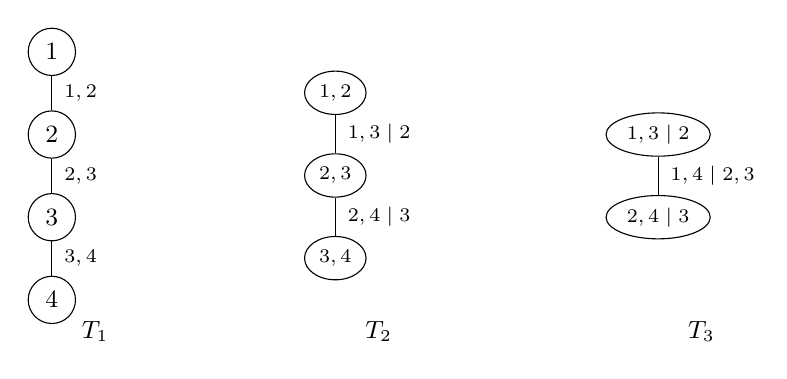
\begin{tikzpicture}[
      x=1cm, y=1cm,
      n1/.style = {circle, draw, minimum size=6mm, inner sep=0pt, font=\small},
      n2/.style = {ellipse, draw, minimum height=5.5mm, inner sep=2pt, font=\scriptsize},
      el/.style = {font=\scriptsize, inner sep=1.5pt, fill=white},
      tl/.style = {font=\itshape\small},
    ]
    \node[tl] at (0.55, -3.55) {$T_1$};
    \node[n1] (x1) at (0,  0)    {1};
    \node[n1] (x2) at (0, -1.05) {2};
    \node[n1] (x3) at (0, -2.10) {3};
    \node[n1] (x4) at (0, -3.15) {4};
    \draw (x1) -- node[el, right=1mm] {$1,2$} (x2);
    \draw (x2) -- node[el, right=1mm] {$2,3$} (x3);
    \draw (x3) -- node[el, right=1mm] {$3,4$} (x4);

    \node[tl] at (4.15, -3.55) {$T_2$};
    \node[n2] (e12) at (3.6, -0.52) {$1,2$};
    \node[n2] (e23) at (3.6, -1.57) {$2,3$};
    \node[n2] (e34) at (3.6, -2.62) {$3,4$};
    \draw (e12) -- node[el, right=1mm] {$1,3 \mid 2$} (e23);
    \draw (e23) -- node[el, right=1mm] {$2,4 \mid 3$} (e34);

    \node[tl] at (8.25, -3.55) {$T_3$};
    \node[n2] (f13) at (7.7, -1.05) {$1,3 \mid 2$};
    \node[n2] (f24) at (7.7, -2.10) {$2,4 \mid 3$};
    \draw (f13) -- node[el, right=1mm] {$1,4 \mid 2,3$} (f24);
  \end{tikzpicture}
  \caption{A vine on four variables.  Nodes of tree $T_{t+1}$ are edges of
  $T_t$, and edges are labelled by their conditioned and conditioning sets.
  Each edge carries one pair copula, so this vine has
  $4 \cdot 3 / 2 = 6$ of them.}
  \label{fig:vine}
\end{figure}

\subsection{Discrete and mixed variables}\label{sec:discrete-model}

When $X_j$ is not continuous, \eqref{eq:sklar} no longer determines $C$
uniquely, and the density in \eqref{eq:vine} must be replaced by a difference.
Write $u_j = F_j(x_j)$ and $u_j^- = F_j(x_j^-)$ for the right and left limits
of the marginal distribution function.  For a bivariate block in which both
variables are discrete, the contribution to the likelihood is the probability
that the copula assigns to a rectangle,
\begin{equation}\label{eq:pdf-dd}
  \frac{C(u_1, u_2) - C(u_1^-, u_2) - C(u_1, u_2^-) + C(u_1^-, u_2^-)}
       {(u_1 - u_1^-)(u_2 - u_2^-)},
\end{equation}
and when only the second is discrete it is a difference of an h-function,
\begin{equation}\label{eq:pdf-cd}
  \frac{h_{1 \mid 2}(u_1, u_2) - h_{1 \mid 2}(u_1, u_2^-)}{u_2 - u_2^-}.
\end{equation}
The h-functions themselves acquire analogous forms when the conditioning
variable is discrete.  Propagating this through \eqref{eq:vine} requires
carrying, alongside each conditional distribution function
$C_{j \mid D}(u_j \mid \bu_D)$, its value at the left limit of the
\emph{conditioned} variable, $C_{j \mid D}(u_j^- \mid \bu_D)$.  The likelihood theory is due to
\citet{panagiotelis2012} and its use for model selection to
\citet{panagiotelis2017}; \citet{stober2015} treat the mixed
discrete--continuous case.  Section~\ref{sec:vartypes} describes how the
package asks the user for this information --- once --- and what it does with
it.

We treat a third variable type: a continuous variable with an atom at zero, for
which $P(X_j = 0) > 0$ and $X_j$ is continuous on $(0, \infty)$.  Such
variables are ubiquitous in insurance and hydrology.  They are handled by the
same left-limit machinery, with $F_j(x_j^-) = F_j(0) - P(X_j = 0)$ at zero and
$F_j(x_j^-) = F_j(x_j)$ elsewhere; \citet{funk2026} give a recent application
of zero-inflated vines to climate model output.

\subsection{Vine distributions}\label{sec:vinedist-model}

Combining \eqref{eq:sklar} with \eqref{eq:vine} gives a model for the joint
distribution of $\mathbf{X}$ on its original scale: a vine copula for the
dependence, and $d$ univariate distributions for the margins.  We call this a
\emph{vine distribution}.  Estimation proceeds in two steps: fit the margins,
transform the data to the copula scale by the fitted marginal distribution
functions, then fit the vine copula.  This is the two-step estimator of Section~\ref{sec:pcc}: inference for margins
\citep{joe1996ifm, joe2005} when the margins are parametric, and the
semiparametric pseudo-likelihood estimator of \citet{genest1995} when they are
estimated nonparametrically, which is the default.  Its asymptotic properties
for vines are studied by \citet{haff2013} and, in growing dimension, by
\citet{gauss2026}.

%% ===================================================================
\section[The vinecopulib engine]{The \pkg{vinecopulib} engine}\label{sec:engine}
%% ===================================================================

\pkg{rvinecopulib} ships \pkg{vinecopulib} in its entirety as a header-only
\proglang{C++17} library, compiled into the package at installation time.  The
same headers are used, unmodified, by the \proglang{Python} interface
\pkg{pyvinecopulib} \citep{pyvinecopulib}; \pkg{rvinecopulib} vendors the upstream headers unmodified, so the two
interfaces compute identical numbers whenever they ship the same engine
version.  External dependencies are obtained
through \proglang{R}: linear algebra from \pkg{Eigen} \citep{eigen} via
\pkg{RcppEigen} \citep{bates2013}, graph algorithms from \pkg{Boost.Graph} \citep{siek2002} and quadrature and
special functions from \pkg{Boost.Math}, weighted rank correlations from
\pkg{wdm} \citep{wdm},
and threading from \pkg{RcppThread} \citep{RcppThread}.  The \proglang{R}--%
\proglang{C++} boundary is \pkg{Rcpp} \citep{eddelbuettel2011} and consists of
33 functions, each of which converts an \proglang{R} list to a
\proglang{C++} object, makes one library call, and converts back.

This section describes the parts of the design that a reader needs in order to
understand why the workflows of Section~\ref{sec:usage} are computationally
feasible.  It is not an API reference; the library documentation at
\url{https://vinecopulib.github.io/vinecopulib/} serves that purpose.

\subsection{Structure representation and the computation index}\label{sec:decomposition}

The core data structure is the regular vine.  \pkg{vinecopulib} stores it in
\emph{natural order}: the anti-diagonal of the R-vine matrix is held separately
as a permutation \code{order}, and the remaining entries are relabelled so that
the anti-diagonal of the relabelled array reads $1, \dots, d$.  The off-diagonal entries live in a
triangular array whose row $t$ has $d-t$ entries.  Truncation is then a
resize of that array: it is $O(1)$ and it frees the memory of the discarded
rows, which matters when $d$ is large and the fitted model is sparse.

The reason for this layout is not storage but computation.  Consider evaluating
\eqref{eq:vine}.  Tree $t$ needs, for each of its edges, two conditional
distribution functions produced in tree $t-1$.  Two facts about that
requirement are fixed by the structure alone, independently of the data and of
the pair copulas:

\begin{enumerate}
  \item \textbf{Which stored value each edge reads.}  For edge $e$ in tree $t$,
        one argument is always the h-function computed at position $e$ of the
        previous tree; the other comes from a position determined by a running
        column minimum of the structure array.  \pkg{vinecopulib} precomputes
        that minimum array once and every algorithm indexes into it directly,
        replacing a search with a lookup.
  \item \textbf{Which h-functions are needed at all.}  Each edge of tree $t$
        can produce two h-functions, \eqref{eq:hfunc}, but a given one is
        consumed by a later tree only if the structure says so.
        \pkg{vinecopulib} precomputes two boolean masks, one per h-function,
        and every algorithm guards its computation on them.
\end{enumerate}

How much this saves depends on the structure, and it is worth being precise
because the saving is often assumed to be larger than it is.  Writing the
fraction of h-functions that some later tree consumes as $\phi$, a C-vine has
$\phi = 1/2$ exactly in every dimension, so half the work is avoided.  For
regular vines drawn uniformly at random we measure
$\phi \approx 0.58$ at $d = 5$, $0.61$ at $d = 10$, $0.60$ at $d = 20$ and
$0.57$ at $d = 50$, a saving of roughly two fifths.  A D-vine is the
unfavourable case: $\phi$ rises from $0.67$ at $d = 5$ to $0.96$ at $d = 50$,
because in a path each interior edge feeds two successors.  The masks therefore
help most for the structures that selection actually produces and least for
D-vines in high dimensions, where the benefit of the index is the avoided
bookkeeping rather than avoided arithmetic.  The replication script reproduces
these figures.

The consequence is that a vine structure carries with it a complete index of
the computation it implies.  \emph{Every} algorithm in the library --- the
density, model fitting, simulation, the Rosenblatt transform and its inverse,
and the analytic derivative cascade of Section~\ref{sec:deriv-engine} ---
traverses the vine with the same two-line dispatch and the same guards.  This
has two benefits beyond speed.  Peak memory is $O(nd)$ rather than $O(nd^2)$,
because the working matrices hold one column per edge of the current tree
rather than the whole cascade; and adding a new algorithm means writing the
per-edge arithmetic, not re-deriving the traversal.
Figure~\ref{fig:decomposition} illustrates the resulting pattern for $d = 5$.

\begin{figure}[t!]
  \centering
  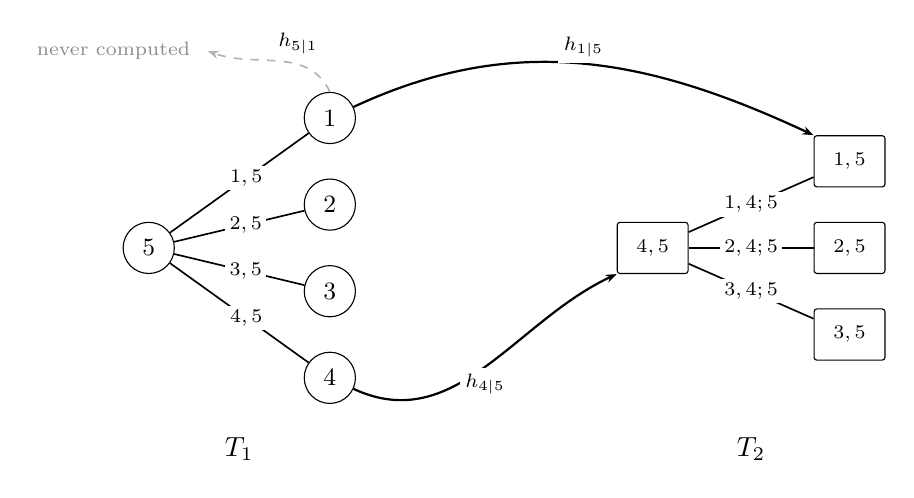
\begin{tikzpicture}[
      x=1cm, y=1cm,
      vtx/.style   = {circle, draw, minimum size=6.5mm, inner sep=0pt, font=\small},
      box/.style   = {rectangle, rounded corners=1pt, draw, minimum height=6.5mm,
                      minimum width=9mm, inner sep=1pt, font=\scriptsize},
      edg/.style   = {draw, semithick},
      used/.style  = {-{Stealth[length=4pt]}, draw, thick},
      skip/.style  = {-{Stealth[length=4pt]}, draw=black!30, dashed, semithick},
      el/.style    = {font=\scriptsize, inner sep=1.5pt, fill=white},
      hl/.style    = {font=\scriptsize, inner sep=2pt, fill=white},
      tl/.style    = {font=\itshape},
    ]
    %% ------------------------------------------------ tree 1 (star on 5)
    \node[tl] at (1.15, -2.55) {$T_1$};
    \node[vtx] (a5) at (0, 0) {5};
    \node[vtx] (a1) at (2.3,  1.65) {1};
    \node[vtx] (a2) at (2.3,  0.55) {2};
    \node[vtx] (a3) at (2.3, -0.55) {3};
    \node[vtx] (a4) at (2.3, -1.65) {4};
    \draw[edg] (a5) -- node[el, pos=0.55] {$1,5$} (a1);
    \draw[edg] (a5) -- node[el, pos=0.55] {$2,5$} (a2);
    \draw[edg] (a5) -- node[el, pos=0.55] {$3,5$} (a3);
    \draw[edg] (a5) -- node[el, pos=0.55] {$4,5$} (a4);

    %% ------------------------------------------------ tree 2 (star on 4,5)
    \node[tl] at (7.65, -2.55) {$T_2$};
    \node[box] (b45) at (6.4, 0) {$4,5$};
    \node[box] (b15) at (8.9,  1.10) {$1,5$};
    \node[box] (b25) at (8.9,  0.00) {$2,5$};
    \node[box] (b35) at (8.9, -1.10) {$3,5$};
    \draw[edg] (b45) -- node[el, pos=0.5] {$1,4;5$} (b15);
    \draw[edg] (b45) -- node[el, pos=0.5] {$2,4;5$} (b25);
    \draw[edg] (b45) -- node[el, pos=0.5] {$3,4;5$} (b35);

    %% ------------------------------------------------ what is passed forward
    \draw[used] (a1) to[out=25, in=155]
      node[hl, above, pos=0.5] {$h_{1|5}$} (b15.north west);
    \draw[used] (a4) to[out=-25, in=-155]
      node[hl, below, pos=0.5] {$h_{4|5}$} (b45.south west);
    \draw[skip] (a1.north) to[out=115, in=-20]
      node[hl, above right, pos=0.55] {$h_{5|1}$} (0.75, 2.5);
    \node[font=\scriptsize, text=black!45, anchor=east] at (0.65, 2.5) {never computed};
  \end{tikzpicture}
  \caption{The computation implied by a five-dimensional C-vine, showing its
  first two trees.  Nodes of $T_2$ are edges of $T_1$.  Each edge of $T_1$
  could supply two conditional distribution functions, but $T_2$ reads only one
  of them; the other, drawn dashed, is never evaluated.  For a C-vine this
  holds at every edge of every tree, so exactly half of the h-function
  evaluations are avoided.  Only two of the four transfers are drawn.}
  \label{fig:decomposition}
\end{figure}

\subsection{Pair copulas}\label{sec:bicop-engine}

A pair copula is represented by a class \code{Bicop} that holds a pointer to a
family implementation, a rotation, and the types of its two variables.  Family
implementations expose only stateless evaluation leaves --- density,
distribution function, the two h-functions and their inverses --- and are
written for unrotated, continuous arguments.  Three concerns are handled once,
above them:

\begin{description}
  \item[Rotation.] Data are rotated before reaching the family and the result
        is mapped back afterwards, so no family implements rotations.  Adding
        a rotation-aware family costs nothing.
  \item[Variable types.] The differences \eqref{eq:pdf-dd} and
        \eqref{eq:pdf-cd} are formed by the layer above the family, from calls
        to the same unrotated leaves.  No family implements discreteness.
  \item[Parameter broadcasting.] Every leaf receives its parameters as an
        $m \times p$ matrix with $m \in \{1, n\}$: either one parameter vector
        broadcast to all observations, or one row per observation.  A model
        whose parameters vary with covariates or with time
        \citep{patton2006, almeida2012, vatter2018} is therefore evaluated by
        exactly the same code as a fixed one, at no cost to the fixed case.
\end{description}

Thirteen families are implemented; Table~\ref{tab:families} lists them.  All
are standard \citep{joe2014} except the extreme-value family of
\citet{tawn1988}.  Adding
a parametric family requires supplying the family's own mathematics and one
line in a factory.  For the two largest sub-hierarchies the mathematics needed
is small: an Archimedean family is determined by its generator, its inverse and
its derivative, and an extreme-value family by its Pickands dependence function
and two derivatives; distribution function, density, h-functions and their
inverses are inherited.  If the family does not supply analytic derivatives,
central finite differences are used automatically, so a new family works with
the machinery of Section~\ref{sec:deriv-engine} immediately.

One numerical detail is worth recording because it accounts for a measurable
part of the timings in Section~\ref{sec:bench}.  Elliptical pair copulas
evaluate the standard normal quantile function once per observation per edge,
and it dominates their cost.  \pkg{Eigen} ships a vectorized implementation of
that function but does not advertise it as available for double precision, so
the natural array expression silently falls back to a scalar evaluation per
element.  \pkg{vinecopulib} drives the vectorized kernel directly, which agrees
with the scalar version to about $2 \times 10^{-15}$ and roughly halves the cost
of a Gaussian pair-copula density.

\subsection{Nonparametric pair copulas}\label{sec:tll-engine}

The nonparametric family \code{"tll"} is a transformation local-likelihood
estimator.  Data are mapped to the standard normal scale by the marginal
quantile function, a local polynomial of degree zero, one or two is fitted to
the log-density there by weighted maximum likelihood, and the result is mapped
back.  The transformation idea is due to \citet{geenens2014}; the local-%
likelihood estimator with degrees one and two is that of \citet{geenens2017},
and \citet{nagler2017} add the local-constant variant and study all three in
the vine context.  The bandwidth is a plug-in rule based on the sample
covariance on the normal scale, scaled by a factor depending on the polynomial
degree and adjusted for the strength of dependence.

Two implementation choices matter for what follows.

First, the fitted density is stored on a $30 \times 30$ grid, equally spaced on
the normal scale, and evaluated by interpolation.  Evaluation cost is therefore
independent of the sample size --- a fitted nonparametric pair copula costs the
same to evaluate as a parametric one, which is what makes nonparametric vines
tractable in the first place.  The grid supports not only interpolation but
also the conditional distribution function and its inverse, obtained from
cumulative row integrals and from a closed-form root of the resulting piecewise
quadratic.  These replace, respectively, a repeated numerical integration and a
bisection, and are the source of the largest single speed difference reported
in Section~\ref{sec:bench}.

Second, the estimator reports an \emph{effective} number of parameters: the sum
over the observations of the influence of each point on its own fit
\citep[\S5.3.2]{loader1999}.  This puts the estimator on the same numerical scale as a parametric family's
parameter count, so that the two can be compared under one information
criterion \citep{nagler2017}, and is what allows \code{"tll"} to appear in the
default candidate set rather than being selected by a separate rule.  It is a
practical device rather than a theorem: the criteria retain no exact
justification once a nonparametric candidate enters, and
Section~\ref{sec:app-returns} gives a case where the nonparametric family is
never selected at all.

\subsection{Structure selection}\label{sec:select-engine}

Structure selection follows \citet{dissmann2013}.  Trees are grown one at a
time; within a tree, all edges permitted by the proximity condition are
enumerated, each is weighted by a measure of dependence between its
pseudo-observations, and a maximum spanning tree is extracted.  The trees are
\pkg{Boost.Graph} adjacency lists \citep{siek2002} and the spanning tree is
computed by Prim's or Kruskal's algorithm, or --- for the randomized selection
of \citet{vatter2025} --- by Wilson's loop-erased random walk \citep{wilson1996}.

Two aspects are worth noting.  Edge weights are computed in parallel across
candidate edges and pair copulas are fitted in parallel across the edges of a
tree, with each fit's own thread budget divided down so that the two levels do
not oversubscribe.  And pseudo-observations are freed as soon as the tree that
produced them has been consumed, which is what keeps peak memory at $O(nd)$.

When the truncation level or the dependence threshold is to be selected rather
than fixed, the search is organized as an outer loop over decreasing thresholds
with the modified BIC of \citet{nagler2019} as the criterion.  Pair copulas
whose data have not changed between iterations are not refitted.

\subsection{Derivatives}\label{sec:deriv-engine}

Scores and Hessians of the vine log-likelihood are computed by the cascade of
\citet{stober2013}, using the bivariate derivative formulas of
\citet{schepsmeier2014}.  Because a pair copula in tree $t$ takes as arguments
h-functions that themselves depend on the parameters of trees $1, \dots, t-1$,
differentiating the joint likelihood requires propagating derivatives forward
through the same cascade that produces the density.

\pkg{vinecopulib} builds a derivative cache in a single forward pass over the
vine, guarded by the same masks as Section~\ref{sec:decomposition}, and the
gradient, the joint Hessian and the stepwise Hessian are then read from it
rather than recomputed.  Closed-form derivatives are implemented for every
parametric family, including the two-parameter BB families and the
three-parameter Tawn family, for which they were obtained by symbolic
differentiation of the generator and Pickands calculus and code-generated.
Families without closed forms fall back to central finite differences.  For the
nonparametric family no derivatives are implemented at all: parameter
derivatives are not defined, and rather than silently differentiating an
interpolant the library refuses the request.

\subsection{Correctness}\label{sec:correctness-engine}

Numerical claims in a library of this size need evidence, and
\pkg{vinecopulib} maintains three kinds.  Golden-value tests pin quantities
that have closed forms --- Kendall's $\tau$ of each family, quasi-random number
streams, bivariate normal and $t$ distribution functions --- against references
computed to fifty digits.  Cross-library parity tests call \pkg{VineCopula}
from the \proglang{C++} test suite as a numerical oracle for bivariate
densities, distribution functions, h-functions, inverse h-functions, Kendall's
$\tau$, Blomqvist's $\beta$ and tail dependence coefficients, and for vine
gradients and Hessians.  And a parity harness compares the complete numerical
output of two builds of the library against a tolerance schedule that records,
for each quantity, the tolerance applied and the reason it was relaxed.
Section~\ref{sec:validation} reports what these tests show at the
\proglang{R} level.

%% ===================================================================
\section[Modeling with rvinecopulib]{Modeling with \pkg{rvinecopulib}}\label{sec:usage}
%% ===================================================================

The package exposes three modeling interfaces, one per level of the
construction of Section~\ref{sec:models}.  Each comes as a pair: a constructor
that builds a model from known components, and a fitting function that selects
one from data.  Table~\ref{tab:interfaces} summarizes them.

\begin{table}[t!]
\centering
\begin{tabular}{llll}
\toprule
Level & Data scale & Construct & Fit \\
\midrule
Bivariate copula   & $[0,1]^2$ & \code{bicop\_dist()}   & \code{bicop()} \\
Vine copula        & $[0,1]^d$ & \code{vinecop\_dist()} & \code{vinecop()} \\
Vine distribution  & $\Reals^d$    & \code{vine\_dist()}    & \code{vine()} \\
\bottomrule
\end{tabular}
\caption{The three modeling interfaces.  Objects returned by a fitting function
inherit from the corresponding constructed class, so evaluation, simulation and
plotting behave identically whether a model was specified or estimated.}
\label{tab:interfaces}
\end{table}

The inheritance in the caption is a deliberate simplification of the user's
mental model: \code{bicop()} returns an object of class \code{c("bicop",
"bicop_dist")}, so every method written for a specified model also applies to a
fitted one.  Fitted objects carry the additional information a fit produces ---
the log-likelihood, the number of observations, the controls used --- and
support the standard generics \code{print()}, \code{summary()},
\code{predict()}, \code{fitted()} and \code{logLik()}, and the two copula
levels additionally have \code{plot()} and \code{contour()} methods.  Because \code{logLik()}
returns a proper \code{"logLik"} object with a degrees-of-freedom attribute,
\code{AIC()} and \code{BIC()} work without further code.

\subsection{Bivariate copulas}\label{sec:bicop}

A fixed pair copula is built from a family name, a rotation and a parameter
vector:

\begin{CodeChunk}
\begin{CodeInput}
R> library("rvinecopulib")
R> cop <- bicop_dist("bb1", rotation = 90, parameters = c(3, 2))
R> cop
\end{CodeInput}
\begin{CodeOutput}
Bivariate copula ('bicop_dist'): family = bb1, rotation = 90,
parameters = 3, 2, var_types = c,c
\end{CodeOutput}
\end{CodeChunk}

The distribution functions follow \proglang{R} naming conventions:
\code{dbicop()}, \code{pbicop()} and \code{rbicop()} for the density,
distribution function and random generation, and \code{hbicop()} for the
h-functions \eqref{eq:hfunc} and their inverses.  The dependence summaries are
\code{par\_to\_ktau()}, \code{ktau\_to\_par()}, \code{blomqvist\_beta()}
and \code{tail\_dep()}.

Fitting is done by \code{bicop()}, whose signature is

\begin{CodeChunk}
\begin{CodeInput}
R> args(bicop)
\end{CodeInput}
\begin{CodeOutput}
function (data, var_types = c("c", "c"), family_set = "all", par_method = "mle",
    nonpar_method = "quadratic", mult = 1, selcrit = "aic", weights = numeric(),
    psi0 = 0.9, presel = TRUE, allow_rotations = TRUE, keep_data = FALSE,
    cores = 1)
\end{CodeOutput}
\end{CodeChunk}

The \code{family\_set} argument accepts individual family names or one of
several collective names --- \code{"parametric"}, \code{"nonparametric"},
\code{"archimedean"}, \code{"elliptical"}, \code{"ev"}, \code{"itau"},
\code{"all"} --- with partial matching.  The default \code{"all"} includes the
nonparametric family; as explained in Section~\ref{sec:tll-engine}, its
effective degrees of freedom make this a coherent default rather than an
arbitrary one.  Setting \code{par\_method = "itau"} estimates by inversion of
Kendall's $\tau$ and restricts the candidate set accordingly, with a warning if
the user's set contained families for which this is impossible.  Setting
\code{presel = TRUE} discards candidates whose symmetry properties are
contradicted by the data before any of them is fitted.

Table~\ref{tab:families} lists the implemented families.

\begin{table}[t!]
\centering
\small
\begin{tabular}{llcccc}
\toprule
Family & \code{family} & Par. & Rot. & Tail dep. & Deriv. \\
\midrule
Independence & \code{"indep"} & 0 & --- & none & yes \\
Gaussian & \code{"gaussian"} & 1 & --- & none & yes \\
Student $t$ & \code{"t"} & 2 & --- & both & yes \\
Clayton & \code{"clayton"} & 1 & all & lower & yes \\
Gumbel & \code{"gumbel"} & 1 & all & upper & yes \\
Frank & \code{"frank"} & 1 & --- & none & yes \\
Joe & \code{"joe"} & 1 & all & upper & yes \\
BB1 & \code{"bb1"} & 2 & all & both & yes \\
BB6 & \code{"bb6"} & 2 & all & upper & yes \\
BB7 & \code{"bb7"} & 2 & all & both & yes \\
BB8 & \code{"bb8"} & 2 & all & upper$^\dagger$ & yes \\
Tawn & \code{"tawn"} & 3 & all & upper, asym. & yes \\
Transf. local likelihood & \code{"tll"} & eff. & --- & data-driven & no \\
\bottomrule
\end{tabular}
\caption{Implemented pair-copula families.  Rotations are by 90, 180 and 270
degrees; families marked --- are invariant under them.  The nonparametric
family reports an effective number of parameters
\citep[\S5.3.2]{loader1999}.  Analytic derivatives are used by
\code{scores()} and \code{hessian()}; where they are unavailable the package
falls back to finite differences, except for the nonparametric family, where
derivatives are refused.  $^\dagger$BB8 is tail independent over the interior
of its parameter space; upper tail dependence arises only in the boundary case
$\delta = 1$.}
\label{tab:families}
\end{table}

\subsection{Vine structures}\label{sec:structure-usage}

A vine structure is built from a list of tree arrays by
\code{rvine\_structure()} and from an R-vine matrix by
\code{rvine\_matrix()}.  The two special cases are built from a variable
order by \code{cvine\_structure()} and \code{dvine\_structure()}.  The functions
\code{as\_rvine\_structure()} and \code{as\_rvine\_matrix()} convert between
the two representations, and \code{rvine\_structure\_sim()} draws one at
random.

\begin{CodeChunk}
\begin{CodeInput}
R> structure <- dvine_structure(order = c(3, 1, 4, 2))
R> as_rvine_matrix(structure)
\end{CodeInput}
\begin{CodeOutput}
4-dimensional R-vine matrix ('rvine_matrix')
1 4 2 2
4 2 4
2 1
3
\end{CodeOutput}
\end{CodeChunk}

\code{truncate\_model()} sets all pair copulas above a given tree to
independence.  It has methods for structures, matrices, vine copulas and vine
distributions, and for fitted models it adjusts the recorded number of
parameters and log-likelihood accordingly.

\subsection{Vine copulas}\label{sec:vinecop}

\code{vinecop()} selects and fits a vine copula.  Its arguments fall into four
groups, and it is more useful to describe the groups than to list them.

\emph{What the pair copulas may be}: \code{family\_set}, \code{par\_method},
\code{nonpar\_method}, \code{mult}, \code{presel} and \code{allow\_rotations},
all with the meaning they have in \code{bicop()}.

\emph{How the structure is chosen}: \code{structure} accepts a fixed structure,
a partially specified one --- a $k$-truncated structure fixes the first $k$
trees and leaves the rest to be selected --- or \code{NA} for full selection.
\code{tree\_crit} selects the edge weight, and \code{tree\_algorithm} the
spanning-tree algorithm, with \code{"mst\_prim"} and \code{"mst\_kruskal"}
giving the maximum spanning tree and \code{"random\_weighted"} and
\code{"random\_unweighted"} drawing one at random \citep{vatter2025}.

\emph{How large the model may be}: \code{trunc\_lvl} truncates the vine in the
sense of \citet{brechmann2012} and \code{threshold} sets pair copulas with weak
dependence to independence.  Each accepts a fixed value, or \code{NA} to have it
selected by the modified vine Bayesian information criterion (mBICV) of
\citet{nagler2019}, available as
\code{selcrit = "mbicv"} and as the function \code{mBICV()}, whose prior
probability of non-independence is controlled by \code{psi0}.  \code{selcrit} chooses the criterion used for families.

\emph{Everything else}: \code{weights}, \code{cores}, \code{keep\_data},
\code{show\_trace}, and \code{vinecop\_object}, which refits the parameters of
an existing model while holding its structure and families fixed.

A typical call selects everything:

\begin{CodeChunk}
\begin{CodeInput}
R> u <- pseudo_obs(returns)
R> fit <- vinecop(u, trunc_lvl = NA, selcrit = "mbicv", cores = 4)
R> head(summary(fit), 4)
\end{CodeInput}
\begin{CodeOutput}
 tree edge conditioned conditioning var_types family rotation
    1    1      35, 38                    c,c      t        0
    1    2       19,  4                    c,c      t        0
    1    3      39, 42                    c,c      t        0
    1    4       34,  4                    c,c      t        0
  parameters df  tau loglik
 0.34, 11.02  2 0.22     92
  0.69,  4.71  2 0.48    494
  0.71,  5.25  2 0.50    546
  0.74,  3.67  2 0.53    627
\end{CodeOutput}
\end{CodeChunk}

The \code{summary()} method returns a data frame with one row per pair copula,
so it can be filtered and sorted like any other; printing it also appends a
legend mapping variable indices to names.  The fitted model is inspected
through a family of accessors:
\code{get\_structure()}, \code{get\_matrix()}, \code{get\_pair\_copula()},
\code{get\_family()}, \code{get\_parameters()} and \code{get\_ktau()} for a
single edge, and \code{get\_all\_pair\_copulas()} and its relatives for all of
them at once.

\subsection{Variable types}\label{sec:vartypes}

Discrete and mixed data are the capability that most sharply distinguishes
\pkg{rvinecopulib} from the alternatives, and the design decision that makes
them usable is that the user declares the types once.

At the copula level, types are declared through \code{var\_types}, a character
vector with one entry per variable, \code{"c"} for continuous and \code{"d"}
for discrete.  Evaluating \eqref{eq:pdf-dd} and \eqref{eq:pdf-cd} requires both
$F_j(x_j)$ and $F_j(x_j^-)$, so the data matrix must carry both.  Two layouts
are accepted.  The \emph{expanded} layout has $2d$ columns: the first $d$ hold
$F_j(x_j)$ and the second $d$ hold $F_j(x_j^-)$, with the entries for
continuous variables ignored.  The \emph{compact} layout has $d + k$ columns
where $k$ is the number of discrete variables, and appends left limits only for
those.  The two are interchangeable everywhere --- in \code{bicop()},
\code{vinecop()}, the Rosenblatt transform and conditional simulation --- and
the package converts between them internally.  Note that the types belong to
the model, not to the call: they are given once to \code{vinecop\_dist()} or
\code{vinecop()}, and every later evaluation reads them from the fitted object.

\begin{CodeChunk}
\begin{CodeInput}
R> model <- vinecop_dist(pair_copulas, dvine_structure(1:3),
+    var_types = c("c", "d", "c"))
R> x <- cbind(rnorm(500), rpois(500, 1), rnorm(500))
R> u_expanded <- cbind(
+    pnorm(x[, 1]), ppois(x[, 2], 1), pnorm(x[, 3]),
+    pnorm(x[, 1]), ppois(x[, 2] - 1, 1), pnorm(x[, 3]))
R> u_compact <- u_expanded[, c(1, 2, 3, 5)]
R> all.equal(dvinecop(u_expanded, model), dvinecop(u_compact, model))
\end{CodeInput}
\begin{CodeOutput}
[1] TRUE
\end{CodeOutput}
\end{CodeChunk}

At the vine-distribution level the left limits are computed by the package from
the fitted margins, so the user supplies data on its original scale and
declares types with a single top-level \code{var\_types} argument to
\code{vine()}.  Three types are recognized there: \code{"c"}, \code{"d"} and
\code{"zi"} for a continuous variable with an atom at zero.  Types may also be
carried by the data itself --- an ordered factor is treated as discrete, and a
column wrapped in \code{zero\_inflated()} as zero-inflated --- in which case an
explicit \code{var\_types} that contradicts the data is an error rather than a
silent override.  Unordered factors are expanded into indicator variables.

\subsection{Vine distributions and margins}\label{sec:vine-usage}

\code{vine()} fits a complete multivariate distribution.  Marginal and copula
behaviour are controlled by two lists:

\begin{CodeChunk}
\begin{CodeInput}
R> fit <- vine(
+    dat,
+    margins_controls = list(family_set = "all", selcrit = "bic"),
+    copula_controls = list(family_set = "parametric", trunc_lvl = NA),
+    var_types = c("c", "d", "zi"),
+    cores = 4)
\end{CodeInput}
\end{CodeChunk}

\code{margins_controls} takes three entries.  \code{family\_set} names the
marginal candidates: \code{"kde1d"} for the nonparametric estimator of
\citet{kde1d}, any distribution supported by \pkg{univariateML}
\citep{univariateML}, the aliases \code{"nonparametric"}, \code{"parametric"}
and \code{"all"}, or a user-defined family object as described in
Section~\ref{sec:margin-protocol}.  Candidates may be given per variable, as a
list indexed positionally or by variable name, and each entry may itself be a
vector of candidates.  \code{selcrit} chooses among them by log-likelihood, the Akaike information
criterion (AIC) or the Bayesian information criterion (BIC), with candidates
whose supported types exclude the variable's declared type discarded before
fitting.  \code{cores} controls parallel marginal
fitting, which uses forked processes and is therefore serial on Windows.

Marginal distribution estimation is the one algorithm in the package
implemented in \proglang{R} rather than \proglang{C++}.  Fitted margins are
returned in \code{fit\$margins} and can be examined with the generics of
Section~\ref{sec:margin-protocol}.  One detail is worth knowing when doing so:
an ordered factor is fitted on its integer codes shifted to start at zero, so a
factor with levels $1, \dots, 6$ yields a margin supported on
$\{0, \dots, 5\}$.  \code{margin\_info()} reports that support, and
\code{rvine()} maps simulated values back to the original levels
automatically; only direct calls to \code{dmargin()}, \code{pmargin()} and
\code{qmargin()} see the internal coding.

\subsection{Simulation, conditioning and transforms}\label{sec:sim-usage}

\code{rvinecop()} and \code{rvine()} simulate from a fitted model, on the
copula and the data scale respectively.  Both accept \code{qrng = TRUE} for
quasi-random rather than pseudo-random draws \citep{cambou2017}, and both stay
synchronized with \proglang{R}'s \code{set.seed()}.

Both also perform \emph{conditional} simulation.  The values are supplied through \code{u\_cond} or \code{x\_cond} and the
variables being conditioned on through \code{conditioning\_set}, which accepts
indices or names:

\begin{CodeChunk}
\begin{CodeInput}
R> sim <- rvine(1000, fit, x_cond = c(veh_value = 1.5, agecat = 3),
+    conditioning_set = c("veh_value", "agecat"))
\end{CodeInput}
\end{CodeChunk}

A single vector of conditioning values is recycled to all $n$ draws; an
$n$-row matrix gives observation-specific conditioning, which is what a
predictive distribution over a set of covariate profiles requires.  The model
is reoriented transiently for the purpose and is not modified.

Conditional simulation is efficient when the conditioning variables occupy the
tail of the vine's sampling order, because they then form a self-contained
sub-vine.  \code{vinecop()} therefore accepts a \code{conditioning\_set} argument of its
own, and \code{vine()} accepts one as an entry of \code{copula\_controls}; it
biases structure selection so that the resulting model has this property while
remaining otherwise optimal in the sense of \citet{dissmann2013}.  The algorithm is
described in the companion paper \citep{companion}; the underlying idea of
conditionalizing a regular vine is due to \citet{cooke2015}, and a restricted
version for C- and D-vines to \citet{bevacqua2017}, whose construction is
implemented in the \proglang{Python} package \pkg{VineCopulas}
\citep{claassen2024} from which our implementation was adapted.

\code{rosenblatt()} and \code{inverse\_rosenblatt()} implement the transform of
\citet{rosenblatt1952}, which maps a sample from the model to independent
uniforms and back, and which is the basis of residual diagnostics for vines.
Both accept a \code{conditioning\_set}.  For discrete variables the transform
is not uniquely defined; by default the package randomizes within the atom
\citep{brockwell2007, czado2009}, which yields exactly uniform residuals under
a correctly specified model, and \code{randomize\_discrete = FALSE} returns the
upper endpoint instead.

\subsection{Likelihood derivatives and uncertainty}\label{sec:deriv-usage}

\code{scores()} returns the matrix of observation-wise score contributions and
\code{hessian()} the averaged Hessian, for both bivariate and vine copulas.
Columns are ordered by tree, then edge, then parameter within the pair copula.

The \code{step\_wise} argument distinguishes two objectives.  With
\code{step\_wise = TRUE}, the default, the pseudo-observations entering each
pair copula are held fixed, which is what the tree-by-tree sequential estimator
of Section~\ref{sec:pcc} actually solves; the resulting gradient is close to
zero at a fitted model.  With \code{step\_wise = FALSE} the
derivatives propagate through the h-function cascade, giving the gradient of
the joint log-likelihood, which at a sequentially fitted model is generally not
zero.

From these, \code{vcov()} assembles a covariance estimate, and
\code{confint()} turns it into Wald intervals:

\begin{CodeChunk}
\begin{CodeInput}
R> S <- matrix(0.4, 4, 4)
R> diag(S) <- 1
R> u <- pseudo_obs(matrix(rnorm(800 * 4), 800, 4) %*% chol(S))
R> fit <- vinecop(u, family_set = "parametric", keep_data = TRUE)
R> sqrt(diag(vcov(fit)))
R> sqrt(diag(vcov(fit, step_wise = FALSE)))
R> confint(fit, level = 0.95)
\end{CodeInput}
\end{CodeChunk}

The estimator solves $\bar{s}(\hat\theta) = 0$ with
$\bar{s}(\theta) = n^{-1} \sum_i s_i(\theta)$, so it is an M-estimator, and the
relevant matrices are
\begin{equation}\label{eq:sandwich}
  A = -\frac{\partial \bar{s}(\theta)}{\partial \theta^\top},
  \qquad
  B = n^{-1} \sum_{i=1}^n s_i s_i^\top .
\end{equation}
\code{vcov()} returns $A^{-1} B A^{-\top} / n$, the misspecification-robust
sandwich of \citet{white1982}.  Rows and columns are named by tree, conditioned
pair and conditioning set, so a coefficient can be located in the model without
counting.

The choice of \code{step\_wise} changes what $A$ is, and the distinction matters
enough to state.  With \code{step\_wise = FALSE}, $\bar{s}$ is the gradient of
the joint log-likelihood and $A$ is minus its averaged Hessian: symmetric, and
the classical setting in which $A^{-1} B A^{-\top}$ reduces to the familiar
$A^{-1} B A^{-1}$.  With \code{step\_wise = TRUE} the pseudo-observations
entering each pair copula are held fixed.  That is the estimating equation
sequential estimation actually solves, but it is not the gradient of any
objective: $A$ is a Jacobian rather than a Hessian, and it is block triangular
rather than symmetric.  The sandwich formula still applies --- which is why \eqref{eq:sandwich} is
written with $A^{-\top}$ on the right --- but the information equality $A = B$
does not, so the simpler $A^{-1}/n$ would be wrong here.  That is why the
sandwich is the only form the package offers.

\code{vcov()} treats the copula data as observed, so it quantifies uncertainty
in the pair-copula parameters \emph{given} the margins.  This is the usual
two-stage approximation \citep{joe2005, ko2019}, and its cost is measurable.
The replication material
reports a small experiment: a three-dimensional Gaussian D-vine with
equicorrelation $0.5$, $n = 1000$, 1000 replications, so that a single coverage
proportion carries a Monte Carlo standard error of $0.007$.  Nominal 95\%
intervals attained an average coverage of $0.956$ when the true margins were
used and $0.929$ when they were estimated by ranks; the paired difference is
$0.027$ with a standard error of $0.004$.  The individual per-parameter
proportions are $0.957$, $0.957$, $0.954$ and $0.940$, $0.906$, $0.941$
respectively, but with three parameters and this much Monte Carlo error we
draw no conclusion about which of them suffers most.  What the experiment
supports is the aggregate statement: ignoring marginal estimation makes the
intervals too short, by a small but clearly measurable amount.

That is why \code{vcov()} and \code{confint()} have methods for \code{bicop}
and \code{vinecop} objects but none for \code{vine} objects.  Correcting the
two-stage approximation requires the influence function of the marginal
estimator, and Section~\ref{sec:margin-protocol} makes that estimator a
user-supplied function: there is nothing the package can differentiate.  A
method that silently conditioned on the fitted margins would be
anticonservative by the amount just measured, so we provide none, and document
the bootstrap instead.  The asymptotics of the step-wise estimator in growing
dimension are studied by \citet{gauss2026}.

Lower-level derivative access is available where it is needed to build
something else.  \code{dbicop()} and \code{hbicop()} take a \code{deriv}
argument naming first- or second-order partial derivatives with respect to the
arguments or the parameters, and \code{dvinecop(keep\_all = TRUE)} returns the
per-edge densities and h-functions that the density computation produced
anyway.  Finally, \code{dbicop()}, \code{pbicop()}, \code{hbicop()}, \code{rbicop()} and
\code{dvinecop()} accept a \code{parameters} argument holding one parameter row
per observation, which is what downstream packages modeling covariate-dependent
dependence \citep{vatter2015, vatter2018} require from a vine backend.

%% ===================================================================
\section[Extending rvinecopulib]{Extending \pkg{rvinecopulib}}\label{sec:extend}
%% ===================================================================

Two parts of the modeling pipeline are open to user code: the marginal models
and the criterion by which vine trees are selected.  Both are specified as
protocols --- small sets of generic functions that a user implements for their
own class --- rather than as fixed catalogues of options.  The pattern follows
\pkg{ROI} \citep{theussl2020} and the \pkg{sandwich} decomposition of
covariance estimators into \code{bread()} and \code{estfun()}
\citep{zeileis2006}.

\subsection{The marginal protocols}\label{sec:margin-protocol}

Marginal models enter a vine distribution in two roles: as a \emph{fitted
margin}, which must be evaluated, and as a \emph{family}, which must be fitted
to data before it can be evaluated.  The two roles have separate protocols.

A fitted margin implements four generics.  Three evaluate the distribution ---
\code{dmargin()}, \code{pmargin()} and \code{qmargin()}, dispatching on the
margin rather than on the data --- and the fourth, \code{margin\_info()},
reports metadata: the family name, the variable type, the support, the number
of parameters, and the log-likelihood.  The evaluation methods must be
vectorized and must propagate \code{NA}.

The type reported by \code{margin\_info()} determines how the package computes
the left limit that Section~\ref{sec:discrete-model} requires:
\begin{equation}\label{eq:leftlimit}
  F_j(x^-) =
  \begin{cases}
    F_j(x), & \text{type \code{"c"}},\\[2pt]
    F_j(x - 1), & \text{type \code{"d"}},\\[2pt]
    F_j(0) - P(X_j = 0) \text{ at } x = 0, \quad F_j(x) \text{ otherwise},
      & \text{type \code{"zi"}}.
  \end{cases}
\end{equation}
This is the load-bearing part of the design.  Because the left limit is derived
from the protocol, a zero-inflated margin participates in an ordinary vine with
no special case anywhere in the copula layer: the copula code sees two numbers
per variable and does not know or care how they were produced.

A margin \emph{family} implements two generics: \code{fit\_margin(family, x,
weights, type)}, which returns an object satisfying the fitted-margin protocol,
and \code{margin\_info(family)}, which reports the family name and the variable
types it supports.  A fitter receives weights on every call and must either use
them or reject them explicitly; silently ignoring them would corrupt a weighted
fit without warning.

Two family adapters ship with the package: \code{kde1d\_family()} for
nonparametric margins, with the bandwidth and boundary options of \pkg{kde1d}
as arguments of the family rather than as entries of a control list, and
\code{univariateML\_family()} for the parametric catalogue of
\pkg{univariateML}.  Two further constructors build \emph{fitted} margins
directly, for use when a margin is known rather than estimated:
\code{stats\_margin()} wraps a \pkg{stats} distribution with fixed parameters,
and \code{margin\_dist()} builds one from its density, distribution and
quantile functions.

Writing a family is correspondingly small.  The following implements a
zero-inflated log-normal margin --- a plausible model for insurance claim
amounts, and one no catalogue provides:

\begin{CodeChunk}
\begin{CodeInput}
R> fit_zilnorm <- function(x, weights = numeric(), type = "zi") {
+    if (length(weights) == 0) weights <- rep(1, length(x))
+    pos <- x > 0
+    p0 <- sum(weights[!pos]) / sum(weights)
+    ml <- sum(weights[pos] * log(x[pos])) / sum(weights[pos])
+    sl <- sqrt(sum(weights[pos] * (log(x[pos]) - ml)^2) / sum(weights[pos]))
+    margin_dist(
+      d = function(q) {
+        ifelse(q > 0, (1 - p0) * dlnorm(q, ml, sl), ifelse(q == 0, p0, 0))
+      },
+      p = function(q) {
+        ifelse(q > 0, p0 + (1 - p0) * plnorm(q, ml, sl), ifelse(q < 0, 0, p0))
+      },
+      q = function(p) {
+        ifelse(p <= p0, 0, qlnorm(pmax((p - p0) / (1 - p0), 0), ml, sl))
+      },
+      family = "zilnorm",
+      type = "zi",
+      support = c(0, Inf),
+      npars = 3,
+      loglik = sum(weights[!pos]) * log(p0) +
+        sum(weights[pos] * (log(1 - p0) + dlnorm(x[pos], ml, sl, log = TRUE)))
+    )
+  }
R> zilnorm <- margin_family(fit_zilnorm, family_name = "zilnorm", types = "zi")
\end{CodeInput}
\end{CodeChunk}

The result is a first-class candidate.  It can be used on its own, or placed in
a candidate set where it competes against the built-in families under the
selection criterion:

\begin{CodeChunk}
\begin{CodeInput}
R> fit <- vine(dat, margins_controls = list(
+    family_set = list(claimcst0 = list(zilnorm, "kde1d"), veh_value = "all"),
+    selcrit = "bic"))
\end{CodeInput}
\end{CodeChunk}

\subsection{Custom tree-selection criteria}\label{sec:treecrit}

The edge weight used in structure selection is set by \code{tree\_crit}.  The
built-in choices are Kendall's $\tau$, Spearman's $\rho$, Hoeffding's $D$
\citep{hoeffding1948}, the mutual information of a Gaussian copula, and the
maximum correlation of \citet{renyi1959} estimated by the alternating
conditional expectations algorithm of \citet{breiman1985}.  \citet{czado2013}
compare several of these; the differences are generally small, which is a
reason to make the choice open rather than to enlarge the catalogue.

A function may also be supplied as \code{tree\_crit}.  It is called with a
two-column matrix of pseudo-observations and a vector of weights, and must
return one finite number, whose absolute value is used as the edge strength.  Rows with
missing values or zero weight are removed before the call.  The example below
selects trees by the coefficient of \citet{chatterjee2021}, which detects
functional relationships that rank correlations miss.  Two details of the
contract are worth noticing in it.  The coefficient is deliberately
asymmetric --- it measures how far $Y$ is a function of $X$ --- whereas a tree
edge is undirected, so the callback symmetrizes by taking the larger of the two
directions.  And because no weighted version is implemented here, the callback
rejects weights rather than silently ignoring them, exactly as a margin fitter
must:

\begin{CodeChunk}
\begin{CodeInput}
R> xi_one <- function(x, y) {
+    n <- length(x)
+    r <- rank(y[order(x)], ties.method = "max")
+    1 - 3 * sum(abs(diff(r))) / (n^2 - 1)
+  }
R> xi <- function(data, weights) {
+    if (length(weights) > 0) stop("xi does not support weights")
+    max(xi_one(data[, 1], data[, 2]), xi_one(data[, 2], data[, 1]))
+  }
R> fit_xi <- vinecop(u, tree_crit = xi, family_set = "parametric")
\end{CodeInput}
\end{CodeChunk}

The callback is evaluated on the thread that started the fit, so it need not be
thread-safe; pair-copula fitting within a tree remains parallel.

\subsection{What is not extensible}\label{sec:not-extensible}

Pair-copula families are a closed set.  There is no \proglang{R}-level hook by
which a user can add one, and we do not consider adding one advisable: a family
must supply not only a density but a distribution function, two h-functions,
two inverse h-functions, parameter bounds and a Kendall's $\tau$ map, all of
them called in the innermost loop of every algorithm in the package, and an
\proglang{R} callback in that position would dominate the runtime.  A new
family is a contribution to \pkg{vinecopulib}; as Section~\ref{sec:bicop-engine}
notes, for the Archimedean and extreme-value hierarchies this amounts to a
generator or a Pickands function and its derivatives.  Users needing
data-driven flexibility rather than a specific parametric form are better served
by the nonparametric family, and users needing parameters that vary across
observations by the \code{parameters} argument of Section~\ref{sec:deriv-usage}.

%% ===================================================================
\section{Illustrations}\label{sec:illustrations}
%% ===================================================================

We work through two applications.  The first is continuous and
high-dimensional, and exercises structure selection, sparsity control and the
nonparametric families; it is also the data on which Section~\ref{sec:bench}
reports timings, so that those are measured on a real problem rather than a
synthetic best case.  The second is moderate-dimensional and mixed, and
exercises the marginal protocols, variable types, conditional simulation and
the uncertainty tooling.

\subsection{Financial returns}\label{sec:app-returns}

We begin with the setting vine copulas were developed for.  The
\code{SP500\_const} data of \pkg{qrmdata} record daily closing prices of the
constituents of the S\&P 500 index.  We take the window 2010--2015, keep the 473
series with no missing values, draw a random sample of $d = 50$ of them, and
work with the $n = 1509$ daily log-returns.

\begin{CodeChunk}
\begin{CodeInput}
R> data("SP500_const", package = "qrmdata")
R> prices <- SP500_const["2010-01-01/2015-12-31"]
R> prices <- prices[, colSums(is.na(prices)) == 0]
R> tickers <- sort(sample(colnames(prices), 50))
R> returns <- diff(log(prices[, tickers]))[-1, ]
R> u <- pseudo_obs(as.matrix(returns))
\end{CodeInput}
\end{CodeChunk}

One caveat before any model.  Daily returns are close to uncorrelated but far
from independent: they exhibit volatility clustering, and the standard practice
is to filter each series with a univariate time-series model and fit the vine to
the standardized residuals \citep{dissmann2013}.  We work with the raw returns
because the object of this section is the copula machinery rather than the
marginal dynamics, and nothing below depends on the distinction; a reader
building a risk model should filter first.

Fitting all $50 \cdot 49 / 2 = 1225$ pair copulas without restriction takes
about ninety seconds on four cores and yields a model with 452 parameters, of which
361 pair copulas are not the independence copula.  The interesting question is
whether so large a model is warranted, and the package answers it by selecting
the truncation level under the modified BIC:

\begin{CodeChunk}
\begin{CodeInput}
R> fit <- vinecop(u, family_set = "parametric", trunc_lvl = NA,
+    selcrit = "mbicv", cores = 4)
\end{CodeInput}
\end{CodeChunk}

Table~\ref{tab:modelcomp} compares four fits.  Truncation removes 53 of the 452
parameters and 39 trees at a cost of 504 in log-likelihood.
Figure~\ref{fig:mbicv} shows the whole path, and it needs a word of
explanation, because reading Table~\ref{tab:modelcomp} left to right invites a
wrong conclusion.  The untruncated model has the better modified BIC ($-52247$
against $-51810$), yet \code{trunc\_lvl = NA} returned ten trees.  This is not
a failure of the search: the selection is \emph{sequential}, not a minimization
over truncation levels.  It grows trees one at a time and stops the first time
adding one fails to improve the criterion, exactly as the structure itself is
grown, and it never revisits that decision.  On these data the per-tree gains
are not monotone, so an early flat stretch halts a search that would have
improved again later.

Whether that is the behaviour one wants is a modeling question rather than a
software one.  A sequential rule is cheap and gives a sparse model; a reader who
wants the criterion's minimum over the whole path can compute it directly, as
Figure~\ref{fig:mbicv} does, and pass the result to \code{trunc\_lvl}.  What
matters for reading the table is that the two rows answer different questions.

The third row of Table~\ref{tab:modelcomp} adds the nonparametric family to the
candidate set and returns exactly the parametric fit: at this dimension and
sample size the modified BIC never prefers a nonparametric pair copula at any
edge.  That is a fact about the software's behaviour, not a verdict on
nonparametric estimation, and we return below to the comparison that would
support such a verdict.  The tree criterion matters less than either: switching
Kendall's $\tau$ for the maximum correlation moves the log-likelihood by 2 in
27{,}685.

\begin{table}[t!]
\centering
\small
\begin{tabular}{lrrrrrr}
\toprule
Setting & Trees & Non-indep. & Par. & Log-lik. & BIC & mBICV \\
\midrule
Par., untruncated & 49 & 361 & 452.0 & 28189 & $-53069$ & $-52247$ \\
Par., mBICV truncation & 10 & 312 & 399.0 & 27685 & $-52449$ & $-51810$ \\
All families, mBICV & 10 & 312 & 399.0 & 27685 & $-52449$ & $-51810$ \\
Par., mBICV, \code{mcor} & 10 & 315 & 401.0 & 27687 & $-52438$ & $-51794$ \\
\bottomrule
\end{tabular}
\caption{Fitted vine copulas for 50 S\&P 500 constituents, $n = 1509$.
``Non-indep.'' counts pair copulas that are not the independence copula, out of
1225 for the untruncated model and 445 for the truncated ones.  The third row
adds the nonparametric family to the candidate set and recovers the second row
exactly; see the text, and Table~\ref{tab:heldout} for the comparison that
should be made instead.}
\label{tab:modelcomp}
\end{table}

\begin{figure}[t!]
  \centering
  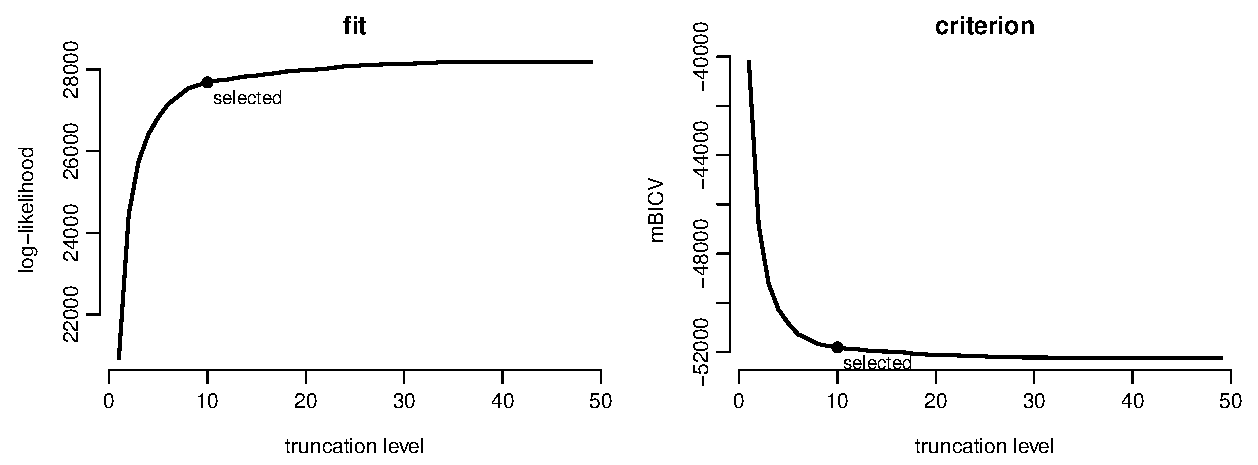
\includegraphics[width=\textwidth]{figures/truncation}
  \caption{Log-likelihood and modified BIC against truncation level for the
  returns data, obtained by truncating the untruncated fit at each level.  The
  filled point marks the level chosen by \code{trunc\_lvl = NA}.  The criterion
  continues to improve beyond it, for the reason given in the text.}
  \label{fig:mbicv}
\end{figure}

The selected model is dominated by the Frank copula (162 of the 312 fitted pair
copulas), followed by the Student $t$ (66) and Gumbel (32).  That the Student
$t$ appears mostly in the first tree and the Frank copula mostly later is the
familiar pattern: tail dependence is a feature of raw returns, and it is largely
accounted for by the time the higher trees are reached.

A word on what these criteria are for, because it is easy to ask more of them
than they can deliver.  AIC, BIC and the modified BIC compare \emph{parametric}
candidates for a given pair copula, using parameter counts that mean the same
thing across candidates.  A nonparametric estimator reports effective degrees of
freedom, which are on a comparable numerical scale but are not parameter counts
in the same sense, and the criteria carry no justification for choosing between
the two on that basis.  The comparison worth making between a parametric and a
nonparametric approach is therefore between whole models, and out of sample.

We split the sample, fit on the first 1000 observations, and evaluate the mean
log-density on the remaining 509:

\begin{CodeChunk}
\begin{CodeInput}
R> train <- u[1:1000, ]; test <- u[1001:1509, ]
R> fits <- list(
+    parametric_itau = vinecop(train, family_set = "itau", par_method = "itau",
+      selcrit = "mbicv", trunc_lvl = NA, cores = 8),
+    parametric_mle  = vinecop(train, family_set = "parametric",
+      selcrit = "mbicv", trunc_lvl = NA, cores = 8),
+    nonparametric   = vinecop(train, family_set = "tll", trunc_lvl = 9, cores = 8))
R> sapply(fits, function(m) mean(log(dvinecop(test, m))))
\end{CodeInput}
\end{CodeChunk}

Table~\ref{tab:heldout} collects the result, with the independence copula as a
baseline.  Two things follow.

The first concerns estimation method rather than family set.  Fitting by
inversion of Kendall's $\tau$ instead of maximum likelihood is more than twenty
times faster --- 1.6 seconds against 37 --- and on these data it also predicts
\emph{better} out of sample, 16.12 against 15.85.  The two-parameter families
that maximum likelihood can reach and $\tau$-inversion cannot buy in-sample fit
that does not survive the split.  For exploratory work at this dimension,
\code{par\_method = "itau"} is the better default, and it is the setting we use
for the timings in Section~\ref{sec:runtime}.

The second concerns the nonparametric family, and it is a caution.  A
nonparametric vine truncated at the same level as the parametric one has
16{,}818 effective degrees of freedom against 1000 training observations, and
it predicts far worse: 8.29 against 16.12.  Truncating it harder helps ---
three trees give 13.33, one tree 11.44 --- but nothing in this family of models
approaches the parametric fit.  That is the expected outcome and not a defect:
kernel estimators need sample sizes that grow with the number of pair copulas,
and $d = 50$ with $n = 1000$ is not that regime.  Nonparametric pair copulas
earn their place in low dimensions, where a misspecified parametric family
costs more than the variance of a kernel estimate; Section~\ref{sec:runtime}
shows what they cost to evaluate once fitted.

\begin{table}[t!]
\centering
\begin{tabular}{lrrrr}
\toprule
Model & Trees & Parameters & Fit (s) & Held-out log-density \\
\midrule
Independence                       & 0 &     0.0 & ---  &  0.00 \\
Parametric, \code{itau}, mBICV     & 9 &   337.0 &  1.6 & \textbf{16.12} \\
Parametric, \code{mle}, mBICV      & 9 &   352.0 & 37.0 & 15.85 \\
Nonparametric, 9 trees             & 9 & 16{,}818.4 &  1.8 &  8.29 \\
Nonparametric, 3 trees             & 3 &  7{,}039.7 &  0.5 & 13.33 \\
Nonparametric, 1 tree              & 1 &  2{,}681.9 &  0.2 & 11.44 \\
\bottomrule
\end{tabular}
\caption{Whole-model comparison on the returns data, $d = 50$: fitted on 1000
observations, evaluated by mean log-density on a held-out 509.  Parameter
counts for the nonparametric models are effective degrees of freedom.  Fitting
times are on eight cores.}
\label{tab:heldout}
\end{table}

\subsection{Insurance claims}\label{sec:app-insurance}

We turn to data of a kind that no other vine implementation in \proglang{R}
can accommodate.  The \code{dataCar} data of \citet{insuranceData} record
67{,}856 one-year motor insurance policies: the claim amount incurred, the
number of claims, the vehicle's value, the fraction of the year the policy was
exposed, and categorical descriptions of the vehicle and the driver.  We take a
random subsample of 10{,}000 policies.

Four of these variables are not continuous, and they are not discrete in the
same way.  Claim cost is continuous on $(0, \infty)$ but has an atom at zero of
mass $0.929$: most policies make no claim.  Vehicle age and driver age category
are ordered factors.  Exposure and vehicle value are continuous.  We exclude the
claim count, because it is positive exactly when the claim cost is positive; a
vine containing both would model a deterministic relationship as a copula, which
no family can represent well.  Deciding which of two structurally linked
variables to keep is an ordinary modeling judgment, and the package will not
make it for the user.

Variable types need not be declared separately when the data carry them.  An
ordered factor is recognized as discrete, and \code{zero\_inflated()} marks a
column as continuous-with-an-atom:

\begin{CodeChunk}
\begin{CodeInput}
R> data("dataCar", package = "insuranceData")
R> idx <- sample(nrow(dataCar), 10000)
R> dat <- data.frame(
+    cost      = zero_inflated(dataCar$claimcst0[idx]),
+    veh_value = dataCar$veh_value[idx],
+    exposure  = dataCar$exposure[idx],
+    veh_age   = ordered(dataCar$veh_age[idx]),
+    agecat    = ordered(dataCar$agecat[idx]))
R> predictors <- c("veh_value", "exposure", "veh_age", "agecat")
\end{CodeInput}
\end{CodeChunk}

The claim cost needs a marginal model that no catalogue supplies.  We use the
zero-inflated log-normal family built in Section~\ref{sec:margin-protocol} and
let the remaining margins be selected from explicit candidate lists: the two
continuous variables from a handful of parametric families and the
nonparametric estimator, the two ordered factors from the nonparametric
estimator alone.  Naming the candidates rather than passing \code{"all"} is
deliberate here.  Vehicle value is recorded to the nearest hundred dollars and
one policy in the subsample carries a recorded value of exactly zero, which
the strictly positive families in the \pkg{univariateML} catalogue --- the
log-normal, gamma, and Weibull among them --- cannot represent; naming the
candidates keeps the selection over families that can.

\begin{CodeChunk}
\begin{CodeInput}
R> fit <- vine(
+    dat,
+    margins_controls = list(
+      family_set = list(
+        cost = zilnorm,
+        veh_value = c("kde1d", "norm", "sstd", "std", "logis", "cauchy"),
+        exposure = c("kde1d", "beta", "norm", "unif"),
+        veh_age = "kde1d", agecat = "kde1d"),
+      selcrit = "bic"),
+    copula_controls = list(family_set = "parametric", selcrit = "bic",
+                           conditioning_set = predictors, keep_data = TRUE),
+    keep_data = TRUE, cores = 4)
\end{CodeInput}
\end{CodeChunk}

The \code{conditioning\_set} argument asks for a structure in which the four
policy characteristics occupy the tail of the sampling order.  This costs
nothing in fit quality --- the selected pair copulas are the same --- but it is
what makes the conditional simulation below reliable rather than a matter of
luck.  Without it, whether a given conditioning set can be conditioned on
depends on the structure the selection happens to return, and a model fitted on
a different subsample may refuse.

Table~\ref{tab:margins} reports what was selected.  The user-defined family wins
for the claim cost, as it must, being the only candidate that can represent an
atom; among the automatically selected margins a skewed Student $t$ is chosen
for vehicle value and a beta distribution for exposure, which is supported on
$(0,1)$.  The two ordered factors are fitted nonparametrically and report
effective parameter counts of $8.28$ and $7.56$.  Figure~\ref{fig:margins}
shows three of the fits.

\begin{table}[t!]
\centering
\begin{tabular}{lllrr}
\toprule
Variable & Type & Selected family & Parameters & Log-likelihood \\
\midrule
\code{cost} & \code{"zi"} & \code{zilnorm} & 3.00 & $-8539.2$ \\
\code{veh\_value} & \code{"c"} & \code{sstd}    & 4.00 & $-13600.9$ \\
\code{exposure} & \code{"c"} & \code{beta}    & 2.00 & $44.6$ \\
\code{veh\_age} & \code{"d"} & \code{kde1d}   & 8.28 & $-13688.5$ \\
\code{agecat} & \code{"d"} & \code{kde1d}   & 7.56 & $-17199.9$ \\
\bottomrule
\end{tabular}
\caption{Selected marginal models for the insurance data.  Types were inferred
from the column classes.  Parameter counts for the nonparametric margins are
effective degrees of freedom.  Exposure has a positive log-likelihood because
its density exceeds one on part of the unit interval.}
\label{tab:margins}
\end{table}

\begin{figure}[t!]
  \centering
  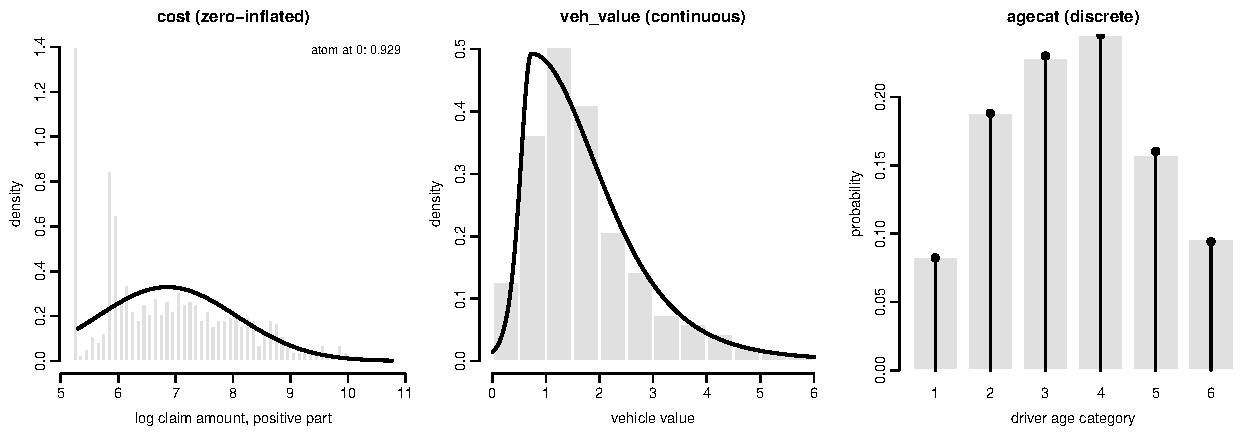
\includegraphics[width=\textwidth]{figures/margins}
  \caption{Three of the five fitted margins.  Left: the positive part of the
  claim cost on the log scale, with the fitted zero-inflated log-normal density
  rescaled to the positive part; the atom at zero carries mass $0.929$.
  Centre: vehicle value with the selected skewed Student $t$ density.  Right:
  the driver age category, with observed relative frequencies as bars and
  fitted probabilities as points.}
  \label{fig:margins}
\end{figure}

The selected vine copula is sparse: three of its ten pair copulas are the
independence copula, and of the remaining seven only two carry appreciable
dependence.  The strongest is vehicle value against vehicle age,
$\hat\tau = -0.517$, fitted by a rotated BB7 copula --- older vehicles are worth
less, which is not news.  The substantively interesting one is exposure against
claim cost, $\hat\tau = 0.356$, fitted by a Joe copula rotated by 180 degrees.
That family is asymmetric with lower tail dependence --- here $0.59$ --- and
the asymmetry is the point: the association between exposure and cost is much
stronger in the lower tail than the upper.  Policies exposed for a small
fraction of the year almost never claim, far more reliably than heavily exposed
policies always do.  A symmetric family would have averaged the two and
described neither.  Everything from tree
two onwards is independent or negligible.  It is worth noting that the modified
BIC would \emph{not} truncate this model --- evaluated along the nested path it
prefers keeping trees two and three by about 35 units --- and that in any case
the conditioning-aware selection used here requires an untruncated vine, so the
two features cannot presently be combined.  Table~\ref{tab:features} lists them
separately for that reason.

\begin{CodeChunk}
\begin{CodeInput}
R> summary(fit$copula)
\end{CodeInput}
\begin{CodeOutput}
 tree edge conditioned conditioning var_types  family rotation
    1    1        1, 3                    d,c     joe      180
    1    2        5, 2                    d,c clayton       90
    1    3        2, 4                    c,d     bb7      270
    1    4        4, 3                    d,c clayton        0
    2    1        1, 4            3       d,d   indep        0
    2    2        5, 4            2       d,d clayton       90
    2    3        2, 3            4       c,c     joe      180
    3    1        1, 2         4, 3       d,c   indep        0
    3    2        5, 3         4, 2       d,c   frank        0
    4    1        1, 5      2, 4, 3       d,d   indep        0
 parameters df    tau loglik
          2  1  0.356  136.0
      0.092  1 -0.044   30.0
   1.2, 2.0  2 -0.517 3005.3
      0.057  1  0.028   10.3
             0  0.000    0.0
      0.075  1 -0.036   14.2
          1  1  0.019    4.9
             0  0.000    0.0
       0.25  1  0.028    8.1
             0  0.000    0.0

---
1 <-> cost,   2 <-> veh_value,   3 <-> exposure,   4 <-> veh_age,
5 <-> agecat
\end{CodeOutput}
\end{CodeChunk}

The \code{var\_types} column shows \code{"d"} where the data declared
\code{"zi"}.  That is the type system working as designed: the third type
exists at the vine-distribution level, where it selects the left limit in
\eqref{eq:leftlimit}, and the copula layer needs only to know whether a
variable has atoms.  \code{vine()} therefore collapses \code{"zi"} to
\code{"d"} before handing the copula its types, and the zero-inflation is
carried entirely by the margin.

Wald intervals for the pair-copula parameters are available even though the
model contains discrete variables, where the backend differentiates by finite
differences rather than in closed form.  They are requested from the copula
component rather than from the fitted distribution, which is the interface
making explicit that they condition on the margins:

\begin{CodeChunk}
\begin{CodeInput}
R> confint(fit$copula)
\end{CodeInput}
\begin{CodeOutput}
             2.5 % 97.5 %
T1.1,3       1.849  2.161
T1.5,2       0.068  0.117
T1.2,4.par1  1.125  1.216
T1.2,4.par2  1.948  2.098
T1.4,3       0.032  0.083
T2.5,4;2     0.046  0.103
T2.2,3;4     1.012  1.056
T3.5,3;2,4   0.128  0.378
\end{CodeOutput}
\end{CodeChunk}

These intervals treat the fitted margins as known, so they understate the
uncertainty by the amount measured in Section~\ref{sec:deriv-usage}.  For this
model the effect is likely larger than in that experiment, because the claim
cost's margin is a three-parameter fit rather than a rank transform.  An
honest interval for the whole distribution requires a bootstrap over both
stages, which the recipe in \code{?parameter\_uncertainty} performs.

The question such a model is fitted to answer is predictive: what claim
distribution should we expect from a policy with given characteristics?  This is
conditional simulation, and it needs no refitting.  Conditioning values are
supplied on the original data scale, in the units the data came in, and the
conditioning variables are named:

\begin{CodeChunk}
\begin{CodeInput}
R> profile <- data.frame(veh_value = 1.5, exposure = 0.75,
+    veh_age = ordered(2, levels = levels(dat$veh_age)),
+    agecat  = ordered(2, levels = levels(dat$agecat)))
R> sim <- rvine(20000, fit, x_cond = profile,
+    conditioning_set = c("veh_value", "exposure", "veh_age", "agecat"))
\end{CodeInput}
\end{CodeChunk}

For this profile --- a mid-value vehicle, two years old, a young driver, exposed
for three quarters of the year --- the simulated probability of a claim is
$0.103$ against an unconditional $0.067$, and the expected cost per policy rises
from $123$ to $196$.  Figure~\ref{fig:condsim} shows why.  The conditioning
raises the probability that a claim occurs by half, but the distribution of the
amount \emph{given} that one occurs barely moves: its median goes from $934$ to
$990$.  Almost all of the change in expected cost is frequency, not severity.
That decomposition is what an insurer wants from such a model, and reading it
off requires a joint model of a zero-inflated variable and a set of mixed
covariates --- which is the case this section was chosen to make.

\begin{figure}[t!]
  \centering
  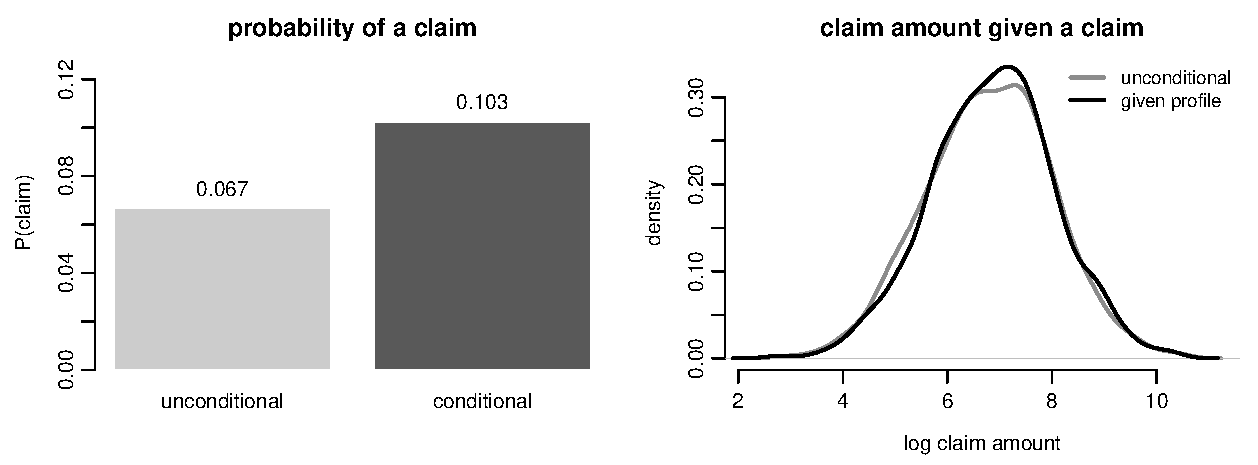
\includegraphics[width=\textwidth]{figures/condsim}
  \caption{Conditional and unconditional predictions from the fitted vine
  distribution, from 20{,}000 draws each.  Left: probability that a policy
  incurs a claim.  Right: the distribution of the claim amount given that a
  claim occurs, on the log scale.}
  \label{fig:condsim}
\end{figure}

%% ===================================================================
\section{Comparison and benchmarks}\label{sec:bench}
%% ===================================================================

This section compares \pkg{rvinecopulib} with the available alternatives.  We
report what the package can do that they cannot, then establish that it
computes the same numbers where a comparison is possible, and only then report
how long it takes.  The order is deliberate: a speed claim from an unvalidated
implementation is worth nothing.

All measurements were made on an idle AMD Ryzen Threadripper 2990WX with 32
cores and 125\,GB of memory, running Ubuntu 22.04 with the reference BLAS,
under \proglang{R}~4.6.1 \citep{R},
\pkg{rvinecopulib}~\pkgversion, \pkg{VineCopula}~2.6.2
\citep{VineCopula}, and \pkg{kdecopula}~0.9.3 \citep{nagler2018jss}.  The
\pkg{VineCopula} build includes two parallelization fixes we contributed while
preparing this comparison, described at the end of
Section~\ref{sec:runtime}; without them its multicore timings measure the
defects rather than the algorithm.

Every timing is the fastest of several repetitions rather than the median.
Anything else running on the machine can only make a repetition slower, so the
minimum is the best available estimate of the uncontended cost, and it also
discards the first-call warm-up.  This matters more than it may appear: medians
of three repetitions moved by up to $37\%$ between two runs of the replication
script on the same machine, while minima are stable to a few percent.

\subsection{Functionality}\label{sec:functionality}

Table~\ref{tab:features} compares capabilities.  We include the two
\proglang{R} packages that fit vine copulas, the two that fit nonparametric
copulas, the archived predecessor, and the actively maintained implementations
in \proglang{Python} and \proglang{MATLAB}.

\begin{table}[p]
\centering
\footnotesize
\setlength{\tabcolsep}{4pt}
\begin{tabular}{lccccccc}
\toprule
& \rotatebox{60}{\pkg{rvinecopulib}}
& \rotatebox{60}{\pkg{VineCopula}}
& \rotatebox{60}{\pkg{kdevine}}
& \rotatebox{60}{\pkg{CDVine}}
& \rotatebox{60}{\pkg{pyvinecopulib}}
& \rotatebox{60}{\pkg{VineCopulas}}
& \rotatebox{60}{\pkg{MATVines}} \\
\midrule
\multicolumn{8}{l}{\emph{Models}}\\
Regular vines                      & \checkmark & \checkmark & \checkmark & --- & \checkmark & \checkmark & \checkmark \\
C- and D-vine constructors         & \checkmark & \checkmark & \checkmark & \checkmark & \checkmark & \checkmark & \checkmark \\
Parametric pair copulas            & 11 & 12 & 12 & 10 & 11 & 6 & 9 \\
Nonparametric pair copulas         & \checkmark & --- & \checkmark & --- & \checkmark & --- & --- \\
Margins fitted jointly             & \checkmark & --- & \checkmark & --- & \checkmark & \checkmark & --- \\
User-defined margins               & \checkmark & --- & --- & --- & \checkmark & --- & --- \\
\midrule
\multicolumn{8}{l}{\emph{Data}}\\
Discrete variables                 & \checkmark & --- & --- & --- & \checkmark & \checkmark & --- \\
Mixed continuous/discrete          & \checkmark & --- & --- & --- & \checkmark & \checkmark & --- \\
Zero-inflated variables            & \checkmark & --- & --- & --- & \checkmark & --- & --- \\
Observation weights                & \checkmark & \checkmark & \checkmark & --- & \checkmark & --- & --- \\
\midrule
\multicolumn{8}{l}{\emph{Selection}}\\
Automatic truncation               & \checkmark & --- & --- & --- & \checkmark & --- & --- \\
Automatic thresholding             & \checkmark & --- & --- & --- & \checkmark & --- & --- \\
Modified BIC                       & \checkmark & --- & --- & --- & \checkmark & --- & --- \\
User-defined tree criterion        & \checkmark & \checkmark & --- & --- & \checkmark & --- & --- \\
Randomized structure search        & \checkmark & --- & --- & --- & \checkmark & --- & --- \\
\midrule
\multicolumn{8}{l}{\emph{Inference and simulation}}\\
Rosenblatt transform               & \checkmark & \checkmark & --- & \checkmark & \checkmark & \checkmark & \checkmark \\
Conditional Rosenblatt             & \checkmark & --- & --- & --- & \checkmark & --- & --- \\
Conditional simulation             & \checkmark & --- & --- & --- & \checkmark & \checkmark & --- \\
Conditioning-aware selection       & \checkmark & --- & --- & --- & \checkmark & \checkmark & --- \\
Analytic scores and Hessians       & \checkmark & \checkmark & --- & --- & \checkmark & --- & --- \\
Standard errors                    & \checkmark & \checkmark & --- & --- & \checkmark & --- & --- \\
Robust (sandwich) covariance       & \checkmark & --- & --- & --- & \checkmark & --- & --- \\
Per-observation parameters         & \checkmark & --- & --- & --- & \checkmark & --- & --- \\
Goodness-of-fit tests              & --- & \checkmark & --- & \checkmark & --- & --- & \checkmark \\
Vuong and Clarke tests             & --- & \checkmark & --- & \checkmark & --- & --- & --- \\
\midrule
\multicolumn{8}{l}{\emph{Implementation}}\\
Compiled backend                   & \checkmark & \checkmark & --- & \checkmark & \checkmark & --- & --- \\
Multithreading                     & \checkmark & --- & --- & --- & \checkmark & --- & --- \\
On CRAN / PyPI                     & \checkmark & \checkmark & \checkmark & --- & \checkmark & \checkmark & --- \\
Peer-reviewed software reference   & --- & --- & --- & \checkmark & --- & \checkmark & \checkmark \\
\bottomrule
\end{tabular}
\caption{Capability comparison.  Counts of parametric pair-copula families
exclude the independence copula and count rotations of a family once; they were
read off each package's own family enumerator.  \pkg{VineCopula} counts one
more than \pkg{rvinecopulib} because it provides two Tawn parameterizations
where we provide one.  \pkg{pyvinecopulib} binds the same engine as
\pkg{rvinecopulib}, so its column is identical by construction; it is shown so
that the \proglang{Python} alternatives can be compared with each other.
\pkg{CDVine} was archived from CRAN in 2020 and \pkg{MATVines}
\citep{coblenz2021} is distributed outside a package repository.  \pkg{VineCopula} additionally provides
goodness-of-fit, Vuong and Clarke tests and an interactive interface, which
\pkg{rvinecopulib} does not; see Section~\ref{sec:summary}.}
\label{tab:features}
\end{table}

\subsection{Numerical validation}\label{sec:validation}

Table~\ref{tab:validation} compares \pkg{rvinecopulib} with \pkg{VineCopula}
on every quantity the two have in common, for all ten shared parametric
families in all admissible rotations --- 31 configurations --- on a fixed
$19 \times 19$ grid of the unit square.  Densities, distribution functions,
h-functions and their inverses, Blomqvist's $\beta$ and the tail dependence
coefficients all agree to between $10^{-16}$ and $10^{-11}$, which is what one
expects of two independent implementations of the same closed forms in double
precision.

\begin{table}[t!]
\centering
\begin{tabular}{lr}
\toprule
Quantity & Largest absolute deviation \\
\midrule
Density                                & $2.0 \times 10^{-14}$ \\
Distribution function                  & $5.6 \times 10^{-16}$ \\
h-functions                            & $4.1 \times 10^{-15}$ \\
Inverse h-functions                    & $3.0 \times 10^{-11}$ \\
Blomqvist's $\beta$                    & $4.4 \times 10^{-16}$ \\
Tail dependence coefficients           & $0$ \\
Kendall's $\tau$, all but Frank        & $9.1 \times 10^{-8}$ \\
Kendall's $\tau$, Frank                & $7.8 \times 10^{-4}$ \\
\bottomrule
\end{tabular}
\caption{Agreement with \pkg{VineCopula} over 31 family-rotation combinations
and a $19 \times 19$ grid.  The Frank entry is discussed in the text.}
\label{tab:validation}
\end{table}

Kendall's $\tau$ is the exception, and it is worth being precise about which
implementation is responsible.  For Frank copulas the two differ by
$7.8 \times 10^{-4}$, far above rounding.  Frank's $\tau$ is
$1 - 4/\theta + 4 D_1(\theta)/\theta$ where $D_1$ is the first Debye function,
which can be evaluated to machine precision by adaptive quadrature.  At
$\theta = 3$ that reference value is $0.307246959431$; \pkg{rvinecopulib}
returns it to $1.1 \times 10^{-16}$ and \pkg{VineCopula} is off by
$7.8 \times 10^{-4}$.  The remaining discrepancies, of order $10^{-8}$ for BB6
and BB8, are of the same character and arise from the quadrature used for
integrals with an endpoint singularity.

Writing this section also turned up a defect on our side.  Joe's Kendall
$\tau$,
\[
  \tau(\theta) = 1 + \frac{2}{2 - \theta}
    \bigl\{ \psi(2) - \psi(2/\theta + 1) \bigr\},
\]
has a removable singularity at $\theta = 2$, where numerator and denominator
vanish together.  The implementation evaluated the quotient directly and
returned \code{NaN} at exactly that point --- reachable in practice, since $\theta = 2$ is an
ordinary interior point that a user may specify directly or arrive at from a
prior fit.  The limit is $1 - \psi'(2) =
2 - \pi^2/6$, and the fix is a series expansion in a neighbourhood of the
singularity; the entry for Joe in Table~\ref{tab:validation} is now exact.
We mention it because it is the kind of defect that a comparison against an
independent implementation finds and a test suite written against one's own
implementation does not.

\emph{Vine log-likelihoods.}  For each cell of the runtime grid below we
verified that the two packages, given the same data and the same matched
settings, select structures with the same log-likelihood.  The check is part of
the replication script and reports on the very fits that were timed, not on a
separate pair fitted for the purpose.  Under maximum likelihood the largest
relative discrepancy was $1.1 \times 10^{-6}$, and the two selected the same
number of non-independent pair copulas in every cell --- 9 of 10 at $d = 5$, 40
of 45 at $d = 10$, and 154 of 190 at $d = 20$.  Under $\tau$-inversion, where
near-ties between families are broken differently, the two do not reach the same
optimum: the gap is $0.5$ at $d = 5$ and grows to $169$ at $d = 50$, or $0.05\%$
to $0.6\%$ of the log-likelihood, always in our favour.  Section~\ref{sec:runtime} returns to what that means for the
comparison.  One restriction must be stated: the two
do not share a convention for the orientation of rotated families, so a vine
containing 90- or 270-degree rotations cannot be constructed identically in
both.  The vine-level comparison is therefore restricted to unrotated and
180-degree families; rotations are covered at the bivariate level, where the
correspondence is unambiguous.

\emph{Nonparametric estimation.}  Section~\ref{sec:runtime} reports the
accuracy comparison against \pkg{kdecopula} alongside the timings, because the
two cannot be read separately.

\emph{Discrete models.}  No alternative implementation exists, so we validate
internally: \eqref{eq:pdf-dd} against direct evaluation of the copula measure
on a rectangle, the empirical Kendall's $\tau$ of simulated data against the
model value, uniformity of the randomized Rosenblatt residuals, and the round
trip \code{inverse\_rosenblatt(rosenblatt(u))} to machine precision.  The
analytic scores of Section~\ref{sec:deriv-usage} were checked against central
finite differences of the vine log-likelihood, agreeing to a relative
$4 \times 10^{-5}$ on a mixed continuous--discrete model.

\subsection{Runtime}\label{sec:runtime}

How much faster \pkg{rvinecopulib} is depends on what is being computed, and
the differences are large enough that a single summary figure would be
misleading.  We separate fitting from evaluation, and within fitting we
separate maximum likelihood from $\tau$-inversion.

\paragraph{Matched settings.}  Against \pkg{VineCopula} we match the setting
exactly: the candidate set is the intersection of the two catalogues, the
selection criterion is AIC, the tree criterion is Kendall's $\tau$, the
independence pre-test is disabled, and no truncation is applied.  We check in every cell that the two implementations
reach a comparable optimum before quoting a ratio.  Under maximum likelihood
the log-likelihoods agree to a relative $10^{-6}$ or better.  Under
$\tau$-inversion they do not agree exactly, because near-ties between families
are broken differently: the relative gap is at most $5.7 \times 10^{-3}$, but
in absolute terms it reaches 33 at $d = 20$ and 169 at $d = 50$, always in our
favour.  We report the ratios anyway, because the gap is between $0.05\%$ and $0.6\%$
of the log-likelihood and the two models are of the same size to within a pair
copula or two: the counts of non-independent pair copulas agree exactly at
$d = 5$ and $d = 10$, and differ by one of 190 at $d = 20$ and by seven of 1225
at $d = 50$.  But the
direction should be stated: we are fitting a marginally better model in
marginally less time, so the $\tau$-inversion rows slightly flatter us, and a
reader should treat them as comparing two implementations of the same procedure
rather than two computations of the same number.

\paragraph{Fitting.}  Table~\ref{tab:runtime} reports structure selection and
estimation.  Two regimes are visible and they say different things.

Under maximum likelihood on a single core the gain is modest and slightly
\emph{decreasing} in dimension: $1.66\times$ at $d = 5$, $1.58\times$ at
$d = 10$, $1.49\times$ at $d = 20$.  This is the honest number for that case and
it is not dramatic: both implementations spend most of their time in compiled
code running the same optimizer over the same families, and there is little to
win.

Under $\tau$-inversion the picture changes, because parameter estimation stops
dominating and the cost moves to the parts \pkg{vinecopulib} parallelizes ---
computing edge weights over all admissible candidate edges, and fitting the
pair copulas of a tree concurrently.  On one core the advantage is remarkably
flat at $1.66\times$ to $1.75\times$ across all four dimensions.  It is the
scaling that differs: on eight cores \pkg{rvinecopulib} is $6.3\times$ faster
than itself at $d = 50$, \pkg{VineCopula} $2.5\times$, so the advantage between
them widens from $1.66\times$ on one core to $4.2\times$ on eight.  In absolute
terms that is a four-and-a-half-second fit against a nineteen-second one.

The comparison inverts at small dimension, and the table shows it rather than
hiding it.  At $d = 5$ \pkg{VineCopula} is slower on eight cores than on one
($1.04$ against $0.41$ seconds), because a tree of five variables does not
contain enough work to repay starting a worker pool and shipping data to it.
\pkg{rvinecopulib} has the same problem in milder form --- $0.18$ against
$0.23$ seconds --- for the same reason: threads are cheaper than processes, but
they are not free.  Neither package should be run on many cores for a problem
this small, and that is a statement about the size of the problem rather than
about either implementation.

\paragraph{A defect we had to fix before we could measure.}  The first version
of this table showed \pkg{VineCopula} getting \emph{slower} as cores were
added --- at $d = 50$, $52$ seconds on one core against $124$ on eight.  That
is a strange enough result to be worth chasing rather than reporting, and it
turned out to have three causes, none of them a property of distributing work
over processes.

The largest is a captured promise.  The tree criterion is built by a helper
that takes the candidate family set as an argument, and the closure it returns
carries that helper's frame as its environment.  Only the AIC and BIC criteria
read the family set, so under the default $\tau$ the argument is never forced,
and the unevaluated promise keeps a reference to the frame of the caller ---
which holds the data.  The criterion is passed to every worker on every
dispatch, and \pkg{parallel} serializes it once per worker: a function that
computes a rank correlation was carrying $7.4$\,MB, six times the size of the
data it was sent alongside.  Forcing the argument reduces it to $6$\,kB.  The
second is that the parallel mapper was bound to the name \code{lapply},
shadowing the base function for the remainder of the enclosing function, so two
subsequent list extractions --- reading one field out of each of $19{,}600$
records --- were dispatched to the worker pool as well; between them they
accounted for $57\%$ of the runtime.  The third is that the routine computing
edge weights received the entire previous tree when it reads seven fields of
it, more than half of the object being fitted pair copulas it never looks at.

With all three repaired the $d = 50$ fit on eight cores falls from $80$ to $12$
seconds, and a $20$-dimensional maximum-likelihood fit scales $4.3\times$ on
eight cores where it had managed $2.9\times$.  Fitted models are unchanged: we
verified that the structure matrix, the families and both parameter matrices
are identical to those of the released version, for both estimation methods and
at more than one core count.  The fixes are contributed upstream
\citep{VineCopulaPR105}, and Table~\ref{tab:runtime} reports the repaired
version, because a timing against the unrepaired one would measure the defect
rather than the design.

We report this at length for two reasons.  A reader who reproduces our table
against a \pkg{VineCopula} release predating the fix will see very different
numbers and deserves to know why.  And the episode is a caution about
benchmarking generally: the original measurement was reproducible, internally
consistent, and wrong about the thing it appeared to establish.

\begin{table}[t!]
\centering
\small
\begin{tabular}{lrrrrrrr}
\toprule
& & \multicolumn{3}{c}{\pkg{rvinecopulib}} & \multicolumn{3}{c}{\pkg{VineCopula}} \\
\cmidrule(lr){3-5} \cmidrule(lr){6-8}
Method & $d$ & 1 core & 4 cores & 8 cores & 1 core & 4 cores & 8 cores \\
\midrule
Maximum likelihood &  5 &  2.22 &  1.18 & --- &  3.68 &  2.45 & --- \\
                   & 10 & 11.34 &  4.48 & --- & 17.91 &  7.73 & --- \\
                   & 20 & 51.81 & 15.82 & --- & 77.01 & 26.80 & --- \\
\midrule
$\tau$-inversion   &  5 &  0.23 &  0.15 &  0.18 &  0.41 &  0.98 &   1.04 \\
                   & 10 &  1.02 &  0.40 &  0.34 &  1.77 &  2.11 &   2.06 \\
                   & 20 &  4.38 &  1.38 &  0.91 &  7.34 &  5.49 &   5.00 \\
                   & 50 & 28.18 &  7.87 &  4.47 & 46.69 & 23.27 &  18.92 \\
\bottomrule
\end{tabular}
\caption{Structure selection and estimation, fastest of repeated fits, in
seconds.
Maximum-likelihood rows use $n = 1000$ and $\tau$-inversion rows the full
$n = 1509$; an em-dash marks a configuration we did not run.
\pkg{VineCopula} parallelizes with socket clusters, and the cost of starting
them and shipping data to the workers is repaid only when there is enough work
per task: under $\tau$-inversion it still loses time at $d = 5$ and $d = 10$,
and only becomes profitable by $d = 20$.}
\label{tab:runtime}
\end{table}

\paragraph{Evaluating a fitted model.}  Fitting is not the only thing one does
with a vine, and for many applications it is not the expensive part: a risk
calculation simulates from a fitted model repeatedly, and a diagnostic
evaluates the Rosenblatt transform.  These operations are pure traversals of the
h-function cascade, which is exactly what the structure index of
Section~\ref{sec:decomposition} was built for.  Table~\ref{tab:evaluation}
reports them.

The single-core column separates the operations into two groups.  Evaluating
the density, the log-likelihood or the Rosenblatt transform is $1.7\times$ to
$2.4\times$ faster; simulation and the inverse Rosenblatt transform, which are
the same computation run backwards through the vine, are a more modest
$1.3\times$ to $1.4\times$.  The gap between the two groups is the h-function
masks doing their work: a forward traversal can skip the conditional
distribution functions no later tree consumes, whereas an inverse traversal
needs its arguments in the other order and has less to skip.

On eight cores the advantage is between $6\times$ and $12.7\times$ and grows with
dimension, since the per-observation batches that the threads divide grow with
it.  Evaluation is where threading pays best: unlike fitting, it has no
sequential dependency between trees to respect, so the whole traversal
parallelizes over observations.  That the two backward operations track each
other to within $0.6\times$ in every cell is what one would expect of two
operations served by the same traversal, and is a useful check that the numbers
are measuring what we think.

\begin{table}[t!]
\centering
\small
\begin{tabular}{lrrrrrrrr}
\toprule
& \multicolumn{2}{c}{$d = 5$} & \multicolumn{2}{c}{$d = 10$}
& \multicolumn{2}{c}{$d = 20$} & \multicolumn{2}{c}{$d = 50$} \\
\cmidrule(lr){2-3} \cmidrule(lr){4-5} \cmidrule(lr){6-7} \cmidrule(lr){8-9}
Operation & 1 & 8 & 1 & 8 & 1 & 8 & 1 & 8 \\
\midrule
Density              & 2.4 &  8.8 & 1.9 & 8.0 & 2.0 & 10.9 & 1.8 & 11.2 \\
Log-likelihood       & 2.4 & 10.3 & 1.8 & 7.2 & 2.0 & 12.7 & 2.0 & 12.1 \\
Rosenblatt           & 2.2 &  7.2 & 1.8 & 7.6 & 1.9 &  8.1 & 1.7 &  9.2 \\
Inverse Rosenblatt   & 1.4 &  6.3 & 1.4 & 6.3 & 1.4 &  9.4 & 1.4 &  9.3 \\
Simulation           & 1.4 &  6.0 & 1.4 & 6.5 & 1.4 &  9.9 & 1.3 &  9.3 \\
\bottomrule
\end{tabular}
\caption{Evaluation on a fitted model, $n = 1509$: speed-up of
\pkg{rvinecopulib} over \pkg{VineCopula}, on one and on eight cores.  Each
package is timed on its own fitted model; the two agree on the log-likelihood
to a relative $6 \times 10^{-3}$ or better.}
\label{tab:evaluation}
\end{table}

\paragraph{Nonparametric pair copulas.}  The only \proglang{R} implementation
of the same estimator is \pkg{kdecopula} \citep{nagler2018jss}, and the
comparison needs two qualifications before any number.

First, the two select the bandwidth by different rules, so they implement the
same \emph{method} rather than the same estimator, and their fits differ.  We
simulated from Clayton copulas and measured the integrated absolute error of
the fitted density against the truth, over 200 replications per cell.  At
Kendall's $\tau = 0.3$ the two are at parity, with \pkg{rvinecopulib} ahead by
$0.8\%$, $2.5\%$ and $1.2\%$ at $n = 500$, $1000$ and $2000$ against Monte
Carlo standard errors of about one point.  At $\tau = 0.6$ \pkg{kdecopula} is
clearly the more accurate, and increasingly so with sample size: our error
exceeds theirs by $17.4\%$, $23.9\%$ and $28.3\%$, with standard errors of
$1.3$, $1.4$ and $1.3$.  Neither rule is uniformly better and we make no claim
that ours is; what matters here is that fitting times are not comparing like
with like, and that under strong dependence our bandwidth rule oversmooths.

Second, and more importantly, speed is not the substance of the comparison.
\pkg{kdecopula} estimates one bivariate copula.  It has no vine, no discrete
data, no h-function cascade and no way to participate in model selection
alongside parametric families.  What \pkg{rvinecopulib} contributes is not a
faster kernel estimator but a nonparametric pair copula that behaves like every
other family in the catalogue --- it can be selected against parametric
candidates, placed at any edge of a vine, and evaluated by the same code as the
rest.

With that said, the evaluation timings are worth reporting, because they are
not subject to the first qualification: they operate on an already fitted model
and measure only the cost of interrogating it.  On $10^4$ points from a fit
with $n = 1000$, \pkg{rvinecopulib} evaluates the density in 0.23\,ms against
11.3\,ms, an h-function in 1.0\,ms against 446\,ms, and an inverse h-function
in 1.3\,ms against 7.4\,s.  The last is a factor of roughly 5600 and is the one
that decides whether a nonparametric vine is usable, because inverse
h-functions are what simulation and the inverse Rosenblatt transform are built
from: a $d = 10$ nonparametric vine needs 45 of them per simulated observation.
The mechanism is in Section~\ref{sec:tll-engine} --- a closed-form root of a
piecewise quadratic against a bisection that re-integrates the interpolation
grid at every step.

\paragraph{What we do not benchmark.}  Four comparisons are deliberately
absent.  We do not benchmark discrete or mixed vines, because no alternative
implements them and a ratio against nothing is not a result.  We do not
benchmark against \pkg{pyvinecopulib}, because it binds the same engine and any
difference measures the language binding rather than the algorithm.  We do not
time conditional simulation against \pkg{VineCopulas} \citep{claassen2024},
the only other implementation that offers it, because it is written in
\proglang{Python}: a ratio would confound the language, the implementation and
the algorithm, and it is the third a reader would want isolated.  And we do
not quote the library's internal benchmarks, which compare
\pkg{vinecopulib}~\vcldversion\ against its own predecessor rather than against
any alternative implementation.

\subsection{Where the difference comes from}\label{sec:why-fast}

The differences reported above have three identifiable sources, all described
in Section~\ref{sec:engine}, and they explain why the two tracks behave so
differently.  In density evaluation, simulation, the
Rosenblatt transform and estimation at a fixed structure, the precomputed masks
of Section~\ref{sec:decomposition} skip the conditional distribution functions
that no later tree consumes.  How much that saves depends on the structure ---
half for a C-vine, about two fifths for a randomly drawn regular vine, and
almost nothing for a D-vine in high dimensions --- so it contributes to the
advantage without accounting for all of it.  (During structure selection the
structure is not yet known, so the masks cannot apply; there the saving comes
from parallelism across candidate edges and from freeing pseudo-observations as
soon as their tree has been consumed.)  In nonparametric evaluation, the
conditional distribution function and its inverse are obtained from cumulative
integrals and a closed-form quadratic root rather than by repeated numerical
integration and bisection.  And in every model containing a Gaussian or Student~$t$ pair copula, the normal
quantile function is evaluated through the vectorized kernel described at the
end of Section~\ref{sec:bicop-engine}.

%% ===================================================================
\section{Summary and limitations}\label{sec:summary}
%% ===================================================================

\pkg{rvinecopulib} makes vine copula modeling in \proglang{R} both faster and
considerably more general than it has been.  The generality comes from three
design decisions: variable types are declared once and respected everywhere, so
discrete, mixed and zero-inflated data are ordinary rather than special;
marginal models enter through protocols rather than a fixed catalogue, so a
user's own distribution is a first-class candidate; and every control that
governs model selection --- the family set, the tree criterion, the truncation
level, the estimation method --- is exposed rather than fixed.  The speed comes
from treating a vine structure as an index of the computation it implies:
computed once, it tells every algorithm what to compute and what to skip, and
it is what makes the parallelism of Section~\ref{sec:runtime} effective.

Several limitations are worth stating explicitly.

\emph{Model assessment.}  The package provides no goodness-of-fit test and no
Vuong or Clarke test for comparing non-nested models, all of which
\pkg{VineCopula} offers.  Our position is that the derivative machinery of
Section~\ref{sec:deriv-usage} is the more useful primitive --- it yields
standard errors, Wald tests and the ingredients of information-matrix tests ---
but a user who wants a bootstrap goodness-of-fit test will not find one here.

\emph{Pair-copula families are closed.}  Section~\ref{sec:not-extensible}
explains why, but the consequence stands: a family not in
Table~\ref{tab:families} requires a contribution to the \proglang{C++} library.

\emph{The simplifying assumption.}  Every model in this paper assumes that a
conditional pair copula does not depend on the value of its conditioning
variables.  \pkg{rvinecopulib} does not fit non-simplified vines.  The
\code{parameters} argument of Section~\ref{sec:deriv-usage} allows evaluation
of a model whose parameters vary by observation, which is the interface a
downstream package implementing conditional dependence needs, but the package
does not itself estimate such models.

\emph{Nonparametric pair copulas need sample size.}  A nonparametric pair
copula has effective degrees of freedom in the tens, so a $d$-dimensional vine
of them has degrees of freedom in the thousands.  Section~\ref{sec:app-returns}
shows the consequence: at $d = 50$ with $n = 1000$ a fully nonparametric vine
predicts far worse out of sample than a parametric one.  They belong in low
dimensions, or with sample sizes that grow with the number of pair copulas.
Relatedly, information criteria compare parametric candidates; choosing between
a parametric and a nonparametric \emph{model} should be done out of sample.

\emph{Derivatives are restricted.}  Closed-form derivatives are available for
continuous, fully parametric models.  With discrete variables the backend falls
back to central finite differences, which is correct but carries the accuracy of
a finite-difference approximation rather than of an analytic formula.  For
nonparametric pair copulas no derivatives are implemented, so \code{scores()},
\code{hessian()} and \code{vcov()} all refuse a model containing one.

\emph{Uncertainty conditions on the margins.}  The covariance estimates of
Section~\ref{sec:deriv-usage} treat the marginal transformation as known.  This
is standard practice, but it is an approximation \citep{joe2005, ko2019}, and it
errs in the direction that matters: the experiment in
Section~\ref{sec:deriv-usage} shows the resulting intervals are too short, by
about three percentage points of coverage in that design.  Because the margin
protocols make the marginal estimator a user-supplied function, the correction
is not available to the package, and \code{vcov()} and \code{confint()} are
therefore offered for a fitted copula but not for a complete vine distribution.
Quantifying uncertainty in the latter requires resampling both stages.

The algorithms that are new in this release --- conditioning-aware structure
selection, nonparametric estimation with mixed data, and the derivative cascade
in its present form --- are developed in a companion paper \citep{companion}.
A \proglang{Python} interface to the same engine, with machine-learning
ecosystem integration, is described separately \citep{pyvinecopulib}.

Several \proglang{R} packages already build on \pkg{rvinecopulib}:
\pkg{vinereg} \citep{vinereg} for D-vine quantile regression
\citep{kraus2017}, \pkg{svines} \citep{svines} for stationary vine time series
\citep{nagler2022}, \pkg{portvine} \citep{portvine} for portfolio risk measures,
\pkg{copulareg} \citep{copulareg} for copula regression, and \pkg{covsim}
\citep{covsim} for simulation with prescribed covariance and margins.  The
observation-specific parameter interface and the marginal protocols were
designed with such downstream use in mind.

%% ===================================================================
\section*{Computational details}
%% ===================================================================

The results in this paper were obtained using \proglang{R}~4.3.3
\citep{R} with \pkg{rvinecopulib}~\pkgversion, which bundles
\pkg{vinecopulib}~\vcldversion.  \proglang{R} itself and all packages used are
available from CRAN at \url{https://CRAN.R-project.org/}.
\pkg{rvinecopulib} is distributed under the GPL-3; the bundled
\pkg{vinecopulib} headers are distributed under the MIT license, which is
compatible with the GPL.  Development takes place at
\url{https://github.com/vinecopulib/}.

%% ===================================================================
\section*{Acknowledgments}
%% ===================================================================

\textbf{[ACKNOWLEDGMENTS]}  We thank the contributors to \pkg{vinecopulib} and
\pkg{rvinecopulib}, and the authors of \pkg{VineCopulas} \citep{claassen2024},
whose conditional sampling and structure selection routines we adapted.

\bibliography{rvinecopulib}

\end{document}
